\documentclass[11pt]{article}
\usepackage[top=1.00in, bottom=1.0in, left=1.1in, right=1.1in]{geometry}
\usepackage{Sweave}
\renewcommand{\baselinestretch}{1.2}
\usepackage{graphicx}
\usepackage{natbib}
\usepackage{amsmath}
\usepackage{gensymb}
\usepackage{parskip}
\usepackage{xcolor}
\usepackage[disable]{todonotes}
\usepackage{lineno}
\usepackage{xr-hyper}
\newcommand{\R}[1]{\label{#1}\linelabel{#1}}
\usepackage{hyperref}
\usepackage[utf8]{inputenc}
\externaldocument{grephonsupp}

\def\labelitemi{--}
\parindent=0pt

\begin{document}

\renewcommand{\refname}{\CHead{}}

% See also: git/grants/crc2023/crc2023app/docs/crc_notes2023more.tex which has some reference notes

\title{Why longer seasons with climate change may \\ not increase tree growth} 
% Climate change highlights fundamental gaps in\\ plant growth $\times$ growing season length relationships  
% Do growing season length and growth relate? \\ And if not, why not? \\ And if we're not sure, why is that?
\author{E.M. Wolkovich$^1$, Ailene K. Ettinger$^2$, Alana Chin$^3$, Catherine J. Chamberlain$^4$,\\ Frederik Baumgarten$^1$, Kavya Pradhan$^{5,6}$, Rub{\'e}n D. Manzanedo$^{7-9}$ \& \\ Janneke Hille Ris Lambers$^7$}
\date{\today}
\maketitle

$^1$ Forest \& Conservation Sciences, Faculty of Forestry, University of British Columbia, 2424 Main Mall, Vancouver, BC V6T 1Z4, Canada\\
$^2$ The Nature Conservancy of Washington, 74 Wall Street, Seattle, WA  USA \\
$^3$ California State Polytechnic University, Humboldt. Department of Biological Sciences. Arcata, CA, USA \\
$^4$ The Nature Conservancy, 334 Blackwell St Ste 300, Durham, NC, USA \\ 
$^5$ Department of Biology, University of Washington, Seattle, WA, 98195 \\
$^6$ Moore Center for Science, Conservation International, Arlington, VA, 22202 \\ % kpradhan@conservation.org
$^7$ Institute for Integrative Biology, ETH Z{\"u}rich, 8092 Z{\"u}rich, Switzerland \\ %
$^8$ Institute of Plant Sciences, University of Bern, Bern, Switzerland \\
$^8$ Oeschger Center for Climate Change Research, University of Bern, Bern, Switzerland \\


%FIXFIX below
\emph{Author contributions:}  All authors conceived of the idea, prepared the literature review, edited the manuscript and contributed to designing figures; in addition EMW wrote the manuscript, AKE, AC, CJC  and EMW synthesized the literature review, RD led developing Fig. 1 and 5, AKE and EMW developed Figure 2, CJC developed Fig 3, AC, RD and EMW led developing Fig. 4. 

% \emph{Data availability:}  No new data, but summarized data from literature review will be posted on KNB.


\newpage
\linenumbers
% We are a review or perspective, see https://www.nature.com/nclimate/content ... either way we need to be 3-5K words
\begin{abstract} % 179 words
A number of recent studies have challenged the assumption that longer growing seasons lead to increased tree growth, raising concerns that forecasts of future climate change---which include increased carbon storage through this assumption---may be overly optimistic. In a review of recent literature, we found that  58\% of studies supported the assumption of increased growth with longer seasons, while 36\% of studies did not. Diverging results remained when holding methodology constant, which suggests the current major challenge is to understand what underlies this widespread variation. Studies have proposed  a suite of hypotheses for why longer growing seasons may not always increase tree growth, including drought-related constraints and internal limits. These hypotheses and their underlying mechanisms, however, were generally tested in different ways by different fields on different species, making comparisons difficult. We outline how bridging these current divides while simultaneously integrating evolutionary history and ecological theory could yield new advances and build a unified model across species for when longer seasons will---or will not---lead to greater growth, with major forecasting implications. 
% While studies have proposed  a suite of hypotheses for why longer growing seasons may not always increase tree growth, including drought-related constraints, internal limits, and methodological differences, comparing support for them is challenging given their diversity and that they were often confined to one sub-field: studies of tree ring growth tended to focus on external drivers, such as drought, while physiological studies of biomass or carbon allocation, tended to focus on internal limits, such as effects of photoperiod. 
% Two alternative endings:
% We argue that bridging disciplinary divides and integrating theory from community and phylogenetic ecology could help develop and test a mechanistic framework for when longer seasons will---or will not---lead to greater growth.
% We outline how bridging current disciplinary divides in hypotheses and methods while simultaneously integrating ecological theory could drive new advances in fundamental biology with major forecasting implications.  %...and help build a mechanistic framework for when longer seasons will---or will not---lead to greater growth, with implications of improve forecasts of forest responses and climate feedbacks in a warmer world.
\end{abstract}
\section*{Introduction} % 3 Jan 2025: 4087 plus Box

The idea that longer growing seasons lead to increased plant growth is an intuitive tenet across multiple fields of biology, including physiology, dendrochronology and ecosystem ecology \citep{nobel1983biophysical,frank2022dendrochronology}. It is also a foundational assumption of many global carbon cycle models \citep[e.g.][]{ito2020global,friedlingstein2022global}. These models project that continued anthropogenic warming will be partly offset by increased carbon sequestration as warming lengthens growing seasons in many forests \citep{friedlingstein2022global}, an assumption supported by ecosystem-scale studies \citep{chen1999effects,keenan2014net,finzi2020}. 

Yet recent work has questioned this longstanding assumption \citep[e.g.][]{dow2022warm,green2022limits,silvestro2023longer}, with potentially large implications for future climate change. % This research suggests that limitations on plant growth mean forests could be limited sinks with increased warming, despite longer growing seasons. 
These recent studies challenge decades of research reporting increased growth with longer seasons, from observations along elevational and latitudinal gradients \citep[][]{myneni1997increased,berdanier2011growing,king2013tree,cuapio2022there}, classic experiments in lab settings \citep{went1957experimental}, to trends in ecosystem fluxes with warming \citep{chen1999effects,keenan2014net,finzi2020}. Proposed mechanisms for the apparent disconnect are diverse (Fig. \ref{fig:hypotheses}), including the complex nature of climate change \citep[e.g. drought or heat stress,][]{dow2022warm} and internal limits on plant growth  \citep{zohner2023effect}. % as well as inconsistent use of growth and growing season metrics and definitions \citep{green2022limits,korner2023four}.
% Studies that Green \& Keenan say no relationship:
	% Fatichi et al. 2014 (opinion)
	% Fatichi et al. 2019 (review)
	% JIang et al 2020 (FACE or sinilar) 

% Our approach spans multiple fields to unify foundational studies with recent research related to anthropogenic warming. Leveraging a systematic literature review, we examine in which methods, species and approaches extended seasons appear to lead to increased growth, and the current proposed hypotheses. 
Here we review how different fields have studied the relationship between growing season length and tree growth to identify the potential mechanisms that unite---and could disconnect---these processes. % Our approach spans multiple fields, from foundational to recent studies.  
Working across multiple definitions of growth and growing season length (see Box),\R{R1growth} we find results that suggest substantial variation in growth $\times$ season length relationships across species. We also find a pervasive disciplinary split between studies, which often test different mechanisms on different species. Current work often implicitly ignores the importance of community and phylogenetic ecology to plant growth \citep[e.g.][]{Grime:1977sw,Webb:2002or,avila2023evidence}, which could aid the search for a universal model when studying different species. We show how increased cross-disciplinary efforts to build a model across species would allow the field to rapidly develop a framework to predict when, where and how climate change may increase tree growth. % with implications both for forecasts of future climate change and fundamental science.
 % JHRL(Nov2023): I know this would make the sentence long, but I want to say that we are primed to get the insights but only if we take the opportunities (lizzie adds: And make the first sentence much more exciting; maybe move up: we highlight critical insights from physiology, community ecology, evolutionary and life history theory that have been unexamined in recent work)

\section*{Evidence that longer seasons increase plant growth, or not}
%  (spanning 36 papers and 59 unique tests or studies; see Supp or Fig/Table)
The idea that time limits growth is a fundamental principle across biology. Many biological processes---including photosynthesis and aspects of growth---are rate-limited, making time a crucial commodity \citep{nobel1983biophysical,cosgrove2005growth,hilty2021plant}. Thus, the hypothesis that longer growing seasons should increase growth is intuitive---and pervasive. 

Foundational evidence comes from spatial clines across elevation and latitude, with growth decreasing alongside growing season length at higher elevations and latitudes (Fig. \ref{fig:gxelev}). Experimentally, this assumption is supported by small-scale field warming studies that find that phenologically advancing species also grow more with warming \citep[][]{Cleland:2012}, while observationally, ecosystem-scale studies have reported a similar positive relationship between season length and carbon fluxes across decades with global warming \citep{keenan2014net} or in years with warm, early springs \citep{chen1999effects}. However, some recent high-profile studies find no support for this relationship \citep{dow2022warm}. These studies, which often focus on inter-annual correlations with metrics of standardized individual tree growth \citep{dow2022warm,silvestro2023longer}, have generated debate about whether future carbon storage forecasts are overestimated and which metrics of growth \citep{green2022limits}, or growing season length \citep{korner2023four}, are relevant (Fig. \ref{fig:defineGSLgrowth}, see Box).\R{R1box0}

Despite this recent debate, we found that longer seasons lead to increased growth in a slight majority of papers spanning  25 years. Though the number of papers directly addressing this topic is small, we found studies have variously found evidence for---or against---the relationship, with no clear pattern by method or year (Fig. \ref{fig:heatmaps} and see `Literature review methods' in Supplement). For example, carbon assimilation studies were evenly split in finding evidence for or against the relationship  (or simply not testing it, Fig. \ref{fig:heatmaps}). Diverging results were consistently found within methods, suggesting the drivers of this variation are likely due to biological mechanisms, not solely inconsistent definitions of growth or growing season length \citep[as some have recently suggested, e.g. ][see also Fig. \ref{fig:defineGSLgrowth}]{green2022limits,korner2023four}. 

Most studies tested the hypothesis that longer seasons with climate change increase growth via either increased time to grow (10 of 36 papers) or because longer seasons are usually warmer (8 papers), although many also considered hypotheses that could disconnect growth from season length. Studies from dendrochronology (the study of tree rings and their dating) and physiology have readily offered explanations for findings that increased growth may not be a universal outcome of longer seasons (Fig. \ref{fig:hypotheses}). External climatic drivers that offset the positive growth effects of longer seasons are often reported in tree ring studies \citep{kolavr2016response,de2022temperature,camarero2022decoupled}. In particular, the hypothesis that higher temperatures paired with lower precipitation produce negative correlations of season length with growth appeared in 58\% of tree ring studies we reviewed (and was only mentioned once outside of these studies, see also Fig. \ref{fig:hypotheses}). In contrast, 43\% of lab experimental and wood phenology (xylogenesis) studies suggested fundamental internal constraints that prevent trees from responding to longer seasons \citep[Fig. \ref{fig:heatmapssupp},][]{cuny2012life,michelot2012comparing,zohner2023effect}. Yet we found that these hypotheses have been tested in radically different ways on different species, never together, and ignore a suite of relevant research from other disciplines. % As we outline below, a single mechanism is unlikely to explain all results, requiring a more unified framework---and tests of it---for progress. 
 
\section*{Controllers on growth $\times$ season length relationships}

% A suite of mechanisms could prevent a universally positive growth $\times$ season length relationship. 
Major mechanisms that could limit or disrupt the positive effects of longer growing seasons generally fall into two categories: (1) external factors, such as drought, which should impact ecosystem-level trends at regional scales, and (2) internal physiological constraints, which some research suggests are either universal across plants \citep[e.g.][]{zohner2023effect}, or species- and population-specific \citep[e.g.][]{soolanayakanahally2013timing}. \R{R2complaint1nonmutexcl}While we address each in turn, these drivers clearly operate together. Further, the importance of internal versus external drivers likely varies by species, highlighting the need to integrate perspectives from community and phylogenetic ecology. 

\subsection*{External drivers}

% \paragraph{Temperature \& moisture} % Abiotic
\R{R2rate1S}Temperature limits many biological processes. Temperatures that are too cool (below 5\degree C for temperate trees) and too warm \citep[an area of active research, but likely between 35-45\degree C;][]{martinez2008hot,cabon2022cross} slow down biological processes and eventually can lead to tissue death \citep[see Fig. \ref{fig:temperaturecomplex},][]{larcher1980,kramer2012book}. Between these upper and lower limits, biological processes underpinning growth generally accelerate such that warming can have a direct effect, by accelerating biological time, up until the maximum rate for that particular process. Assuming a common growth response curve to temperature, possible increased growth should be predictable at an ecosystem level based on the current seasonal temperatures and the amount of warming (Fig. \ref{fig:moraconcept}). 

How much or whether growth increases at all depends on the non-linear effect of temperature on biological processes (Fig. \ref{fig:temperaturecomplex}). At very cool temperatures---such as in early spring---a small increase in temperature may have limited effect \citep[or even increase frost risk through early budburst, Fig. \ref{fig:hypotheses}e,][]{cat2021pep}, while an increase at warmer temperatures---such as those more common in the summer (e.g. 16 to 18\degree C)---could have a larger physiological impact. However, warming that pushes plants beyond their optima, where many biological rates crash, could have large negative impacts \citep{nobel1983biophysical,leuning2002temperature}. Thus, some studies hypothesize that longer seasons effectively only extend the very cool early-season periods and may have no discernible effect on growth (with varying definitions of growth, see Box)\R{R1box1}, while other studies---based on tree rings---suggest that any increases in growth due to longer seasons can be offset by reduced growth due to high summer temperatures \citep[Fig. \ref{fig:hypotheses},][]{gantois2022new,dow2022warm}. In contrast, other researchers argue that warmer temperatures have not yet pushed trees above their optima \citep{schaber2002evaluation}, and instead have driven increases in growth through accelerated rates, rather than longer seasons \citep[e.g.][]{ren2019}, or through a combination of both.\R{R2rate1E}

Positive effects of longer---or warmer---seasons on growth predicted from temperature responses alone, however, could be counteracted by other external drivers. Moisture deficits from reduced precipitation or higher evaporative demand (commonly invoked in tree ring studies, Fig. \ref{fig:hypotheses}) can slow or stall growth. Support for this hypothesis comes from negative correlations between growth and precipitation \citep[or other metrics related to plant access to water in tree ring studies,][]{kolavr2016response,etzold2022number}, and is well supported by physiological observations  that tree water status can be a biophysical limit to growth \citep[i.e., cells cannot expand without sufficient turgor,][]{peters2021turgor,cosgrove2023structure}, though we found few physiological studies on season length that considered this effect (Fig. \ref{fig:heatmaps}). External biotic factors are also shifting with longer seasons---including herbivory, disease and competition\citep{mitton2012mountain,lange2006thresholds,cleland2024effects}---and can limit productivity \citep{sturrock2011climate,la2008forest,senf2017remote}, though they are missing from the current debate on the impacts of longer seasons on growth (we found no mention of them, Fig. \ref{fig:hypotheses}e). 

\subsection*{Internal constraints}
%  \paragraph{Universal limits \& triggers} 
When and how growth is initiated and ceases is under genetic and developmental control, and thus plants' internal programming could limit growth responses to longer seasons \citep{howe2003genotype}. Research has repeatedly shown that populations vary in their growth and its responses to extended seasons (Fig. \ref{fig:hypotheses}d), reflecting differences in genetic and developmental controls that likely evolved to limit tissue loss to rare early or late-season events \citep{mitton2012mountain,lange2006thresholds,cleland2024effects}. Populations often vary predictably in their end-of-season phenology, with more poleward populations tending to stop height growth (budset) earlier using locally adapted photoperiod cues \citep{soolanayakanahally2013timing,aitken2016}. This means longer seasons are generally driven by spring phenology, which appears far more flexible, and has advanced more rapidly than fall events \citep{aitken2016}. Some recent studies suggest novel roles for the summer solstice \citep{zohner2023effect} in setting a fixed universal developmental switch between when warming temperatures hasten or delay leaf senescence, and in determining when warmer temperatures trigger greater reproduction \citep{Journe2024}. % Within populations, individual trees may also vary in how early or late they initiate (spring) or end (fall) growth. This can be driven by a shifting investment to growth, survival and/or reproduction with growth. For example, saplings, for which growth and survival are paramount, tend to both grow more rapidly \citep{hilty2021plant} and have longer seasons relative to adult trees \citep{augspurger2003differences,rozendaal2010tropical,vitasse2014earlier}, which need to also invest in reproduction. % The response of adult trees may then vary depending on their investment in reproduction. 

Trade-offs between vegetative and reproductive investments may produce important growth response differences across years within individuals, as well as between species. Years of high reproductive output can reduce growth \citep{thomas2011bookchptr,hacket2016tree}. For species that mast---producing abundant cones or fruits in only some years---high reproduction could especially impact measures of wood growth. Higher summer temperatures may trigger masting in the following year \citep{hacket2016tree,hacket2016consistent}; if true, then reduced growth in years following warm summers may not indicate temperatures too high for growth, as recent studies have suggested \citep[e.g.][]{gantois2022new,dow2022warm}, but instead shifting investment to reproduction.

\subsection*{Species-level variation}
The effects of these external and internal drivers are likely to vary across species, with species identity strongly predicting variation in growth $\times$ season length relationships \citep[e.g.][]{cuny2012life,michelot2012comparing}. Though this reality was rarely acknowledged in studies we reviewed (Fig. \ref{fig:hypotheses}c), research in dendrochronology, physiology and in phenology often mentions important differences between certain species groups that should affect how longer seasons affect growth. 

The distinct strategies of deciduous versus evergreen species, including in how and when they invest in leaf and shoot elongation versus cambial growth, can affect how they respond to longer seasons. While evergreen species generally leaf out later than deciduous species they can more immediately photosynthesize with earlier springs, though both types of species generally invest in buds (for new leaves, shoots and flowers) in the preceding year. This means neither can rapidly change their investment in leaf area in response to an earlier spring, but both can have multiple flushes of leaves \citep{day2011regulation,soolanayakanahally2013timing}. Wood growth in evergreen species is generally thought to come from current season photosynthesate, while deciduous species may more often use stored carbon resources \citep{gordon1968seasonal,monson2018finding}. These differences would suggest season length by growth relationships
may be most apparent via lagged effects in deciduous species, but this is rarely studied  \citep[and not clearly supported to date][]{coulthard2020limits,klesse2023legacy}. Further, evergreen species are thought to grow more slowly and thus differences due to season length may be harder to detect \citep{waring1979evergreen}.  

\R{R3complaint2S}This division between evergreen and deciduous species hints at a larger suite of traits that predict growth by growing season length relationships among species. Species that budburst earlier and more readily produce additional leaves \citep[e.g., leaf flushes after budset, and other characteristics more common to `indeterminate' species,][]{kikuzawa1982leaf,Lechowicz:1984cr} may grow more with longer seasons (though potentially with a lag, see Box, Fig. \ref{fig:defineGSLgrowth})\R{R1box2} versus those that budburst later and flush new primary growth only once. Similarly, species adapted to cold, dry or high latitude conditions across their range may have different thresholds for when these external drivers limit or promote growth \citep[e.g., some \emph{Populus} and \emph{Quercus} species,][]{soolanayakanahally2013timing,mckown2016impacts,delpierre2017tree,de2022temperature}. Such differences could easily obscure any overall relationship between growth and growing season length. Supporting this possibility, current studies finding divergent results (Fig. \ref{fig:sppfinds}, Fig. \ref{fig:sppphylo}) span a wide range of species (we found  57 species from 26 genera across 36 papers). While this diversity may appear to make identifying a common relationship between growth and growing season length more difficult, it may instead offer the path to an improved framework.\R{R3complaint2E}% JDonJan12: perhaps worth emphasising someplace that if we want to include growth responses in climate models etc. we need a model that can be fit across (all) species ... [I did this below.]

\section*{Building a new framework for growth $\times$ season length relationships} 

%Predicting when and where longer growing seasons will lead to increased growth would benefit from a framework that leverages species variation to understand when external and internal drivers limit growth. 
% ADDCITES: harmonebook
\R{startframework}Useful models of tree growth for climate change forecasting have to include a diversity of different species, while overcoming the challenges of uneven sampling across species and their contrasting responses. Leveraging the diversity of responses observed across species is possible by integrating ecological advances in how species traits and evolutionary history shape species responses to climate change \citep{cornwell2017phylogenetic}. In particular, advances in phylogenetic comparative methods \citep{Webb:2002or} have moved research away from treating species identity as a simple grouping factor where each species is unique (e.g., \emph{Fagus sylvatica} is different from \emph{Quercus robur} and \emph{Pinus sylvestris}) or fits into a limited set of groups (e.g., deciduous versus evergreen) and towards species as suites of correlated observations, separated by their evolutionary distance (\emph{Fagus sylviatica} is much more closely related to \emph{Quercus robur} compared to \emph{Pinus sylvestris}). New models built from these advances can fit data from all species at once and layer in species-level information.  Traits can capture differences in growth strategies while phylogeny can capture additional species differences, which likely capture unmeasured `latent' traits \citep[][]{pearse2019interaction,morales2024phylogenetic}. %Ailene suggests to cut last sentence

In step with these advances, trait ecology has documented leaf and wood economic spectra that suggest major traits to include in these models \citep[with related databases of these traits often available,][]{Chave2009,diaz2016}. These `economics' define a common trade-off along an acquisitive to conservative axis, where some species grow rapidly and more flexibly to take advantage of resources, but are less defended against herbivores and compete poorly at low resource levels, whereas other species compete well at low resource levels, but at the expense of growing slower  \citep[][]{Grime:1977sw,Chave2009,diaz2016}. While these traits likely miss critical components for understanding how growing season length shapes growth, such as when different species invest in shoot and leaf versus wood growth, they provide a baseline from which to build, and a powerful approach to combine data usefully across species. This approach has already been used to identify that early-leafout species often show faster-growing more acquisitive strategies compared to later-leafout species \citep{cleland2024effects}---differences that may also impact how they respond to longer seasons. 
% While evolutionary distance often predict a suite of important species traits---and possibly also unmeasured latent traits (CITES)---ecophylogenetics incorporates both for a more useful and predictive framework.

In addition to naturally organizing species differences, a trait-based phylogenetic comparative approach can help build a more testable and predictable framework. % that can more readily forecast species responses ... 
Because this approach can flexibly fit evolutionary history and traits together, it allows clades or species groupings that respond similarly to emerge from the data and models \citep{davies2019phylogenetically}, versus being a priori grouped or defined. Similarly traits that co-vary with different responses can be more quickly identified \citep[e.g.,][see Fig. \ref{fig:phylomodel}]{willis2008phylogenetic,davies2019phylogenetically}. \R{R2complaint3S}Both of these benefits could help identify which species or traits to focus additional studies on to gain the most insights, while similarly suggesting areas that should be less studied \citep[e.g., traits that may be too confounded with evolutionary history,][]{cornwell2014functional,westoby2023phylogenetically} or outlier species that may not represent most species \citep{morales2024phylogenetic}. This approach may thus redefine debates over which metrics of growth or growing season length are relevant into debates over which metrics are most relevant for which clades and/or traits.\R{R2complaint3E}% CITE BOX?

Importantly, trait-mediated phylogenetic models aid the search a universal model that can be useful for global forecasts of how growing season length influences growth. By effectively assuming one model, which is then shaped by evolutionary history and trait differences to produce the divergent responses observed across species today, this approach yields an overall estimated growth response alongside a response for each species, which can then be variously combined to scale up. For example, species-level estimates combined with data on species abundance across forests \citep[e.g.][]{FIA,fischer2019swiss} could predict larger-scale metrics, such as satellite observations of phenology and productivity.
This framework also provides an organizing method to re-approach the fundamental question of how external and internal drivers shape growth responses to longer seasons, and a way to tackle what we are argue the three most critical questions in this area.\R{R3complaint5Ephylo}
%ADD?! ... If you do different species in different places you're just learning about changes in species composition across space (and population dynamics), which might give you something but won't give you mechanism -- need models like Nacho's and Freckleton's

% Predicting when and where longer growing seasons will lead to increased growth---or not---is possible with focused efforts to partition variation to different drivers in a framework that leverages species variation. 
% Because species diverge strongly in their growth and investment strategies any search for a common model will need to leverage this variation, as opposed to ignore it ... 

\subsection*{What is the scale of variation in growing season length x growth relationships across space and time?}

The idea that growing season length influences plant growth is fundamental to plant biology, but we found it is rarely tested in ways relevant to the current debate (see `Growth $\times$ elevation relationships' in Supplement), providing a major gap that limits progress. While multiple papers report a lack of relationship between growth and growing season length (Figs. \ref{fig:hypotheses}, \ref{fig:heatmaps}), we have no fundamental understanding of what the effect size of this relationship should be, and thus no way to know if we have sufficient power in current studies to detect it. % Additionally, understanding large-scale pattens often improves models of the underlying processes, by finding unexpected trends or highlighting covarying drivers that must be disentangled. % ; for example, it may force a more immediate efforts to tease out effects of growth rates versus longer seasons. 

Identifying the macro-scale pattern of how growth and growing season length relate should be a primary goal, and one that seems broadly tractable. \R{R2rate2S}Tree ring studies designed to leverage latitudinal and elevational gradients in climate could quickly provide the raw data. Research will then need to develop models that tease out the effects of warmer temperatures across the season---likely affecting important biological rates  (Figs. \ref{fig:temperaturecomplex}- \ref{fig:moraconcept})---versus longer seasons. Disentangling these may require focused efforts to understand xylogenesis across species and climates, but doing so across major climatic gradients could make differences more obvious.\R{R2rate2E} Wood growth provides an obvious and tractable baseline from which to set expectations of how much growth can vary across space, and links to existing major datasets (Fig. \ref{fig:itrbdpep}).  Research will also then need to integrate beyond wood growth, including methods to better characterize changes across the leaf, shoot and wood architecture of different species \citep[e.g.,][]{puletti2020lidar,sillett2024ground} and also extending to the complexity of roots \citep{mckown2016impacts,radville2016}. These data can provide a baseline to compare to the scale of shifts over time, which studies of growth $\times$ growing season length to date have focused on (Fig. \ref{fig:heatmaps}), since the same tree rings measured for understanding spatial variation will also capture inter-annual variation. 

% To answer this: go out and observationally measure the same species across latitude or elevation and aim to measure the RATE and TIMING of primary and secondary growth (getting at total SUM across season). 

% Start with tree rings for this and then break it down by types of growth, GSL metrics etc. (Nail this pattern across space and species; and then fit in what we see/expect over time). 

\subsection*{How prevalent are internal constraints across species and populations?}

% Predicting changes in growth in response to longer seasons requires understanding how much variation is possible inter-annually, within individuals. 
New evidence suggests inter-annual variation in growth may be limited because of internal constraints that prevent plants from fully using longer seasons \citep{zohner2023effect}. If true, this would have major ramifications for how much we expect growth to shift with warming. All plants are limited by internal constraints and how quickly they can build new tissues \citep{marchand2021timing,luo2024internal}, but selection towards different growth strategies (e.g., acquisitive versus conservative) should drive variation in these constraints across species. Selection should also drive local adaptation in these constraints at the population-level \citep{mckown2016impacts,soolanayakanahally2013timing}, by favoring individuals that match to local environmental optima \citep{Colautti:2010,mckown2014np}. This appears to be the case for budset---which indicates the end of height growth, though we currently have data on only a few species \citep{aitken2016,zeng2024weak}. Further, new studies could rapidly test for constraints across species and populations, to work towards a predictive framework using phylogeny and traits to predict these constraints. This approach has already yielded useful insights in spring phenology, highlighting which environmental factors consistently drive budburst across species while also showing widely-cited results may not extend beyond one well-studied species \citep{morales2024phylogenetic}. % Further, many results often schmear across species and populations \citep[e.g., studies using NDVI,][]{zohner2023effect}, but new studies could rapidly test for 

\subsection*{How do external drivers and internal constraints act together?}

% Most research on how growth impacts growing season length with climate change has been focused on either external or internal drivers. Certain studies have documented potential constraints while others focused on teasing out how temperature, drought and other external forces impact growth. Inherently, however, external and internal factors are interconnected and thus any useful model must include both together.  We argue that understanding the pattern across space---and using it benchmark the possible magnitude of inter-annual responses---alongside documenting the scale of internal constraints across species and populations will be critical to help compare responses of external and internal drivers. As these new data come together with trait-mediated phylogenetic models, we expect real advances will require more experiments across scales and disciplines.  

\R{R3complaint1S}The external and internal factors that affect how longer seasons impact growth are inherently interconnected \citep{nobel1983biophysical}. While research often acknowledges this, modeling these together will require both experiments and observational studies, ideally designed to integrate into trait-mediated phylogenetic models. Studies across space could provide some inference by studying how growing seasons measured by vegetative versus wood phenology vary---and attributing variation through models that nest species within populations and include traits while also testing for how climate drives growth.  

% But it needs a lot more work to understand if (a) it is common across species, and populations (partition variance) and (b) holds up under different definitions of GSL (c) is backed up experimentally (Figure showing what we expect from experiments maybe?).

The complexity of climate change and plant growth in response to longer, warmer seasons makes experiments vital to building useful mechanistic models for forecasting. Observational data---used mainly to date to tackle this question (Figs. \ref{fig:heatmaps}, \ref{fig:heatmapssupp})---generally confounds multiple external drivers, including season length, temperature and precipitation regimes \citep{ren2019,ipcc2021,camarero2022decoupled}, making it impossible to tease out actual drivers behind observed trends. \R{R3complaint5S1}Experiments, in contrast, can provide more robust tests. While juvenile stages of trees are often more flexible than their adult forms, they still usually provide predictable inference in differences across species and populations, and so should be integrated far more into studies of how season length affects growth. Using saplings and controlled environments could quickly test how much growth can shift with longer seasons---providing a potentially standardized way to compare constraints across species and populations---and then layer on shifts in external drivers. % Such studies could also begin to tease out effects of increased growth rates due to warmer temperatures versus longer seasons. 

\R{R2rate3S}In particular, mechanistic models will need to tease out changes in season length from warming that affects rates; a challenge best addressed by new experiments that decouple these two factors. Such experiments could start on juvenile trees to help inform the underlying model, select representative species to focus on, and  develop predictions for large-scale studies. Experiments could also inform a better model of lag effects across species, with small-scale studies sampling saplings multiple years after manipulations (versus the common practice of destructive sampling at the end of the treatment growing season) and large-scale studies following existing efforts to test for ecological `memory'  \citep[e.g. ][]{flinker2021promise,schweiger2022transgenerational,chinmemory}. These efforts should help bridge across the contrasting timescales of current physiological and dendrochronological studies of growing season length: we found most physiological studies of growth $\times$ growing season length relationships studied 1-2 years of dynamics, usually of juvenile trees, while tree ring studies focused on synthesizing across decades of adult tree growth.\R{R2rate3E}

\R{R3complaint5S2}Expanding studies across more species will be critical for useful models that can forecast at relevant scales and to help design large-scale experiments. While experimenting on adult trees is difficult, previous challenges in climate change research have led to large-scale experiments to understand other complex drivers \citep[e.g. SPRUCE, DroughtNet, Pfynwald,][]{norby2011ecological,hanson2017attaining,smith2016drought}. We expect similar experiments will be critical here. Preparing for these large experiments using trait-mediated phylogenetic models to understand responses across species, however, could advance new experiments well beyond past efforts \citep{morales2024phylogenetic}. By informing which species or clades to study, new experiments could span enough phylogenetic and trait diversity to forecast to species beyond the experiment and maximize the information gained \citep{cadotte2017phylogenies}.\R{R3complaint1E}

\emph{Conclusions:} 
Anthropogenic climate change has often been described as an unfortunate and unplanned experiment. Like many experiments, it has highlighted important biology we do not know well. Understanding when, how and why longer seasons lead to increased tree growth requires an interdisciplinary reckoning with how temperature, time and a suite of external and internal drivers affect plant growth across species. A mechanistic understanding of how these drivers integrate over species diverse growth strategies and the imprints of evolutionary history to affect growth today is possible, but will require new approaches.  Starting now to leverage data across species to inform and design new large-scale studies and experiments be critical for accurate models of future forest and related carbon dynamics, with implications for projections of carbon sequestration and carbon markets. 

% My version: The task may seem large, but bridging across theory and data from dendrochronology, physiology, community and phylogenetic ecology could rapidly advance fundamental biology in ways that translate directly to improved models of future forest dynamics, with implications for and projections of carbon sequestration and carbon markets as well.  And that includes carbon sequestration---which, we really need now! 

% Ailene's version: Understanding when, how and why longer seasons lead to increased tree growth requires an interdisciplinary reckoning with how temperature, time and a suite of external and internal drivers affect plant growth. A mechanistic understanding of how these drivers integrate to affect growth will be critical for generating accurate global carbon forecasts biophysical feedbacks from future climate change, with implications for and projections of carbon sequestration and carbon markets as well. 

% Most fields studying growth $\times$ growing season length relationships consider a limited set of metrics and a small subset of possible drivers (see Figs. \ref{fig:heatmaps}, \ref{fig:heatmapssupp}). Beyond failing to test a suite of highly relevant mechanisms, the lack of interdisciplinary study means we lack coherent tests that compare multiple mechanisms. Taken together, the current landscape of research suggests we may be testing hypotheses for how plants shift with climate change that we never previously understood well in fundamental biology.
% Most fields studying this include a limited set of metrics and consider only a small subset of potential factors, with entire suites of hypotheses missing from the literature (see Fig. XX). 

% Beyond failing to test a suite of highly relevant mechanisms, the lack of interdisciplinary study means we lack coherent tests that compare multiple mechanisms. Dendrochronology considers almost exclusively external climatic drivers, while physiological tests of constraints do not usually predict for which species, when and where constraints will be most important. Taken together, the current landscape of research suggests we may be testing a hypothesis for shifts with climate change that we never previously understood well in fundamental biology. 

\emph{Acknowledgements:} B. Wuu for extracting growth $\times$ elevation data; R. Z{\"a}ch for logistical support; N. Pederson for discussion, J. Davies and three reviewers for comments that improved the manuscript. % R. Manzanedo was supported with funding from the Swiss State Secretariat for education, Research and Innovation (SERI) by a SERI-funded ERC Starting Grant #MB23.00011 % My Rubel and NSERC funding ...


\clearpage
\section{References}
\bibliography{..//bibtex/grephonbib}
\bibliographystyle{/Users/Lizzie/Documents/git/bibtex/styles/besjournals.bst} % pnas.bst says 87 refs on 18 May 2024


\clearpage
\section{Figures}
% 30 May 2024: Ruben updated figures to make them look better. I have kept the new paths and left the old paths below so we have them.



\begin{figure}[h!]
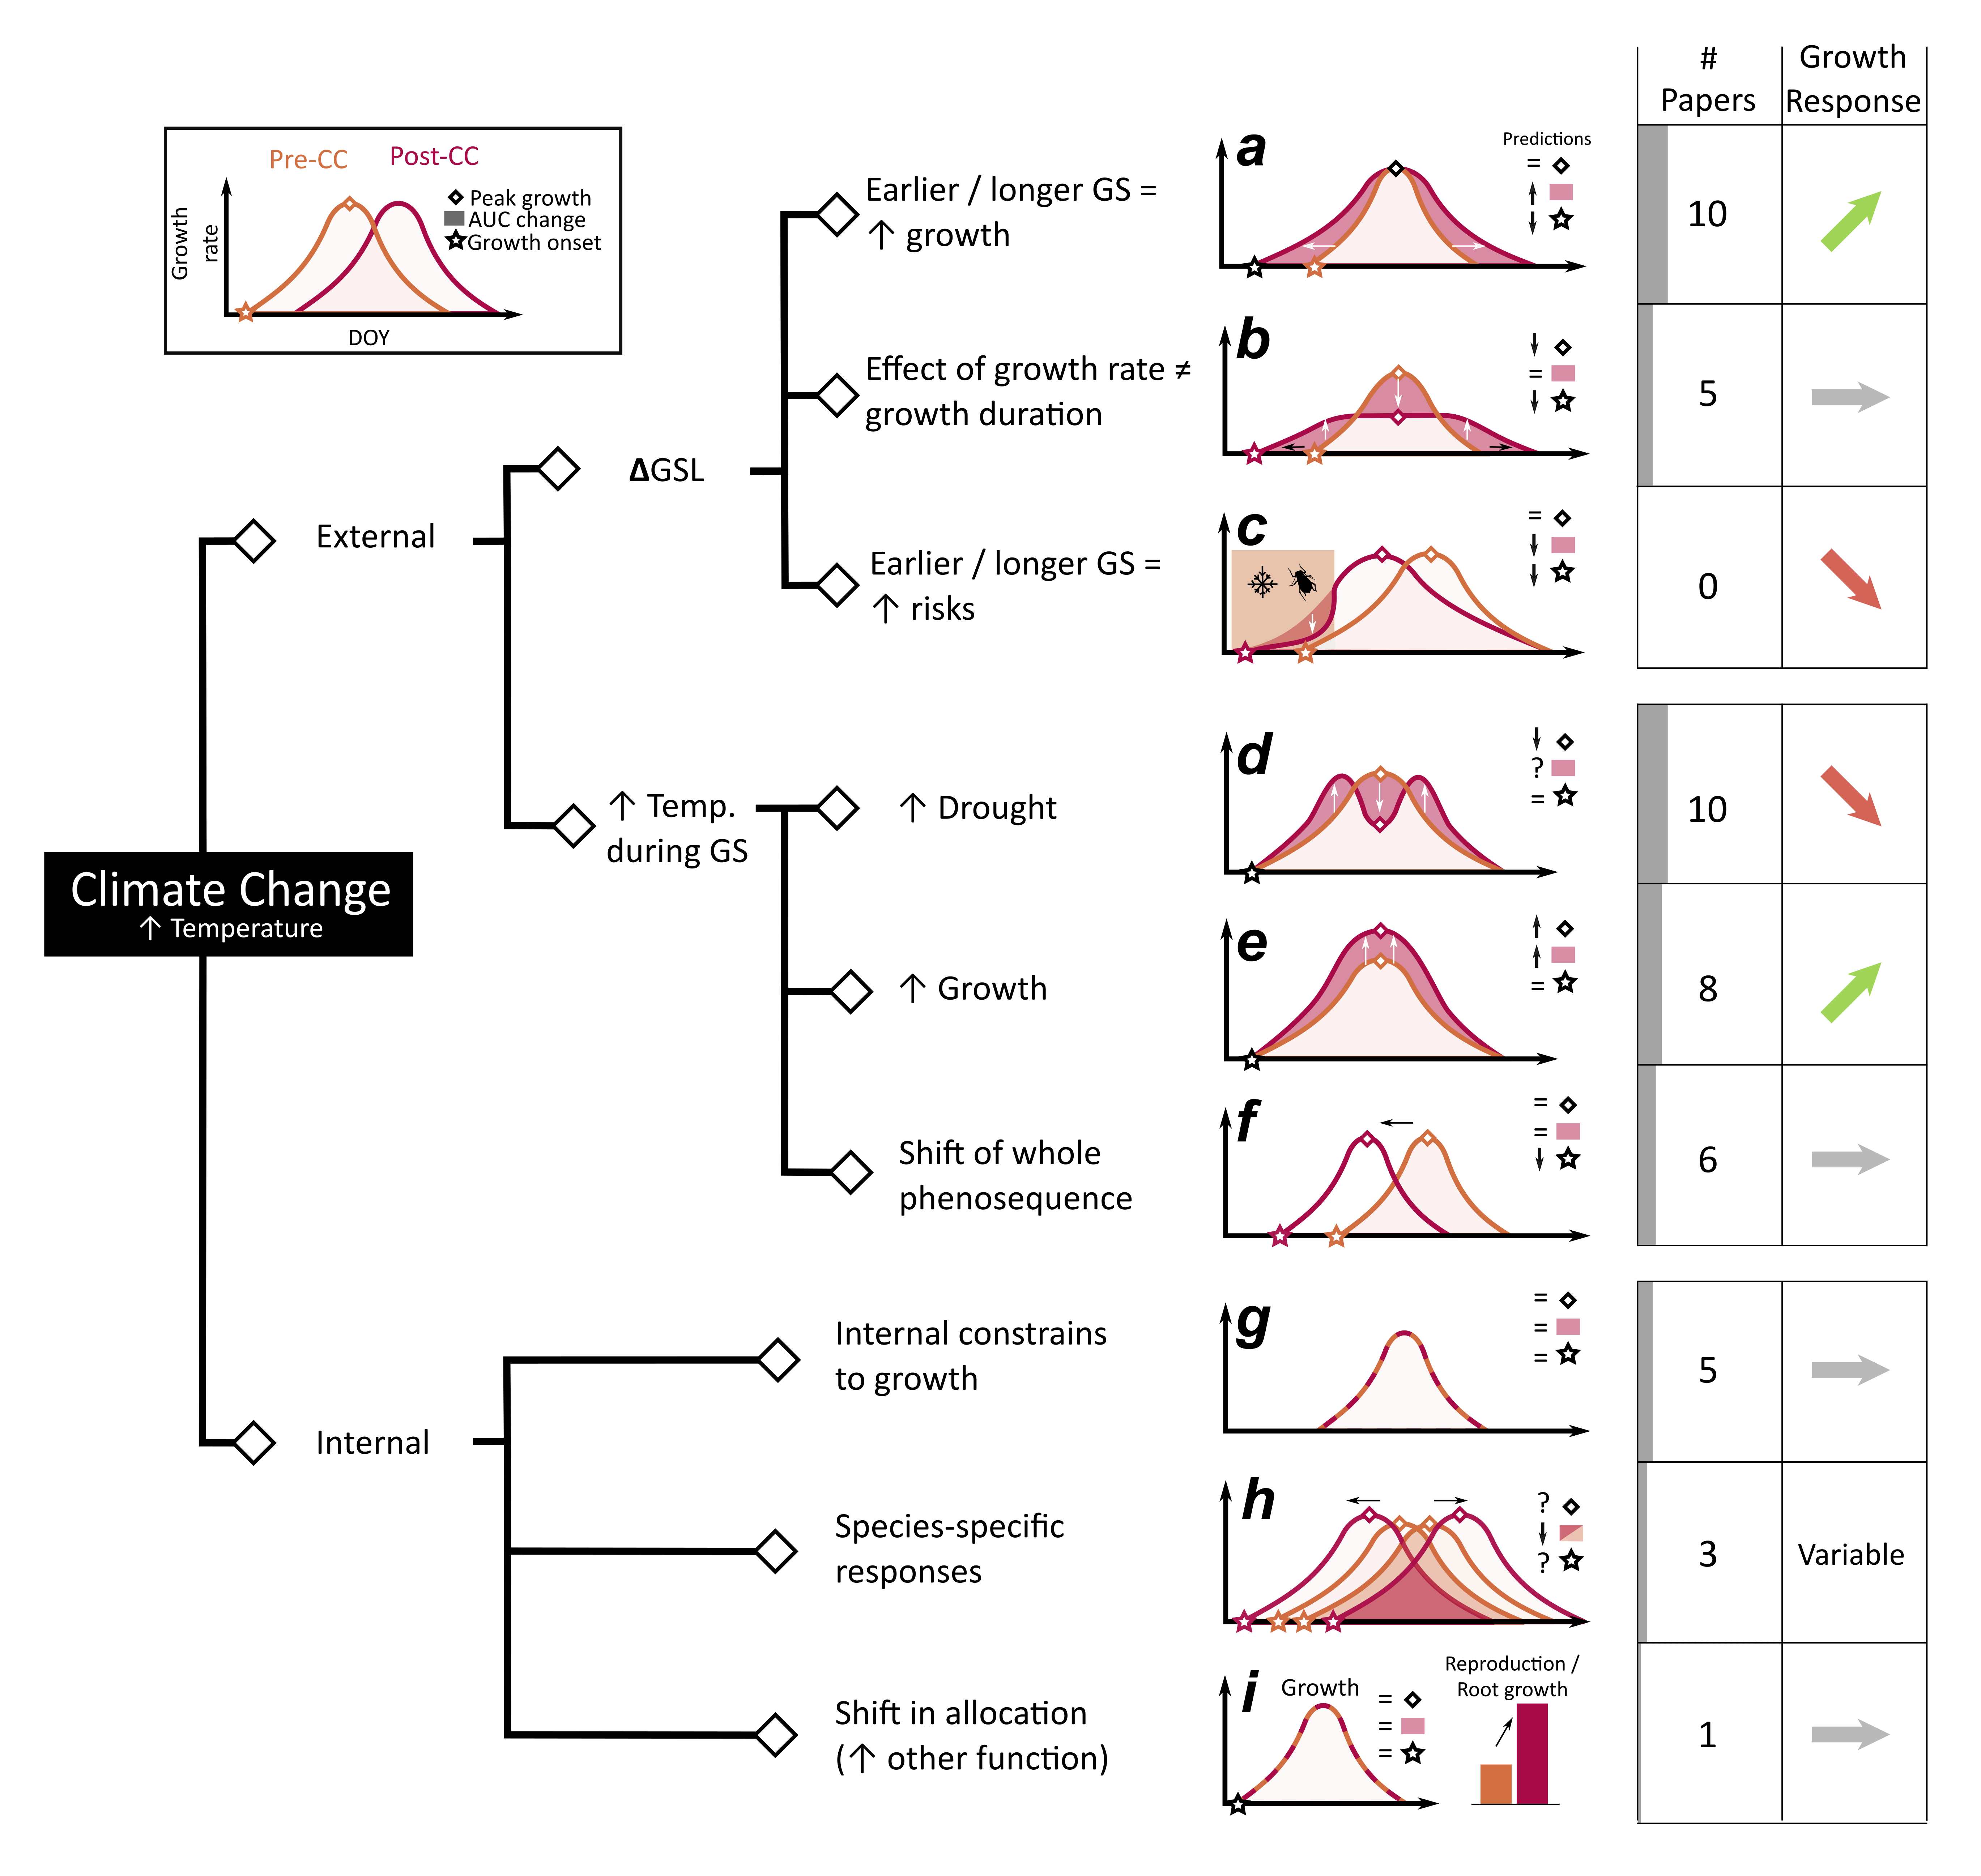
\includegraphics[width=0.9\textwidth]{..//figures/_figuresFromRuben/conceptual.png}
\caption{Climate change may alter growing season (GS) length, which can then affect growth through diverse pathways. We review hypotheses for these pathways showing the number of papers (from a review of papers studying growth $\times$ growing season length) that mentioned each hypothesis (width of the shaded areas of left column is proportional to the number of papers with the number also given, right column shows the expected growth response for each hypothesis). We group hypotheses as focused on mechanisms moderated by the environment (`external') versus those focused on internal physiological constraints, which span both source (photosynthesis-limited) and sink limitation, and could act together. For more details, see Supplement.} 
\label{fig:hypotheses}
\end{figure}

\begin{figure}[h!]
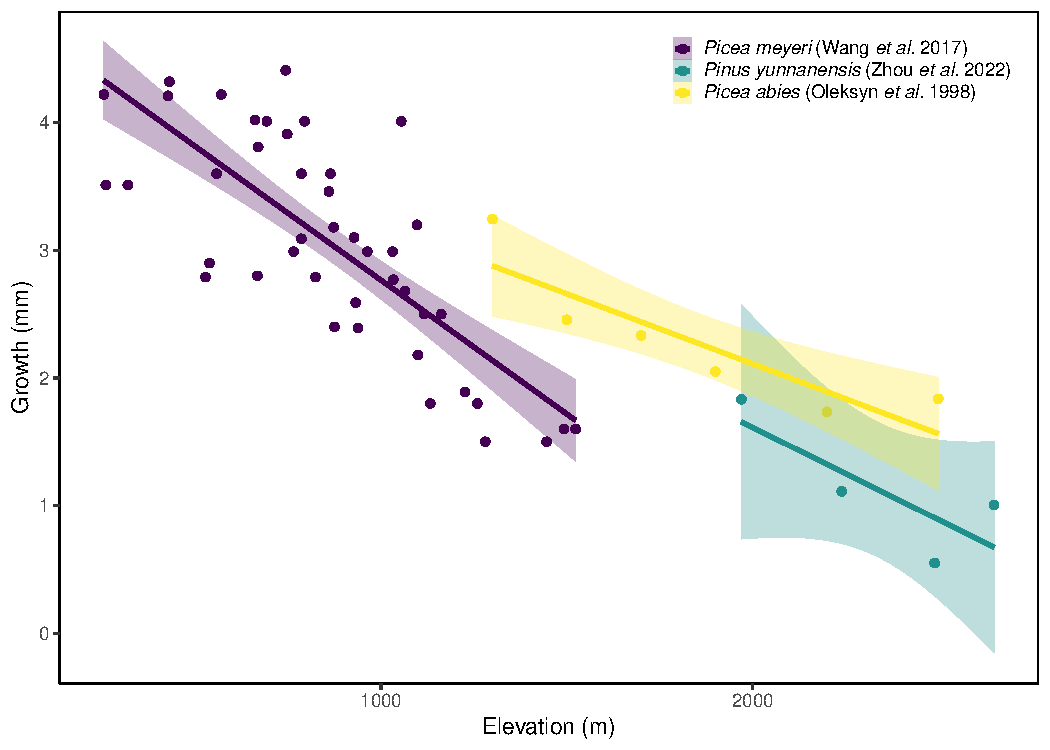
\includegraphics[width=0.7\textwidth]{..//analyses/growthxelevationetc/figures/growthbyelevation_plot.pdf} % {..//figures/_allfiguresFromRuben/growthbyelevation.png}   
\caption{Growth $\times$ elevation relationships from the literature with simple linear regression fits shown with 89\% confidence intervals. \citet{oleksyn1998growth} measured growth (mm) as diameter at breast height increments, while the other studies \citep{wang2017climatic,zhou2022altitudinal} measured growth (mm) as ring width. See Supplement for more methods details.} % and Fig. \ref{fig:growelevMORA} for an example from one site.
\label{fig:gxelev}
\end{figure}

\begin{figure}[h!]
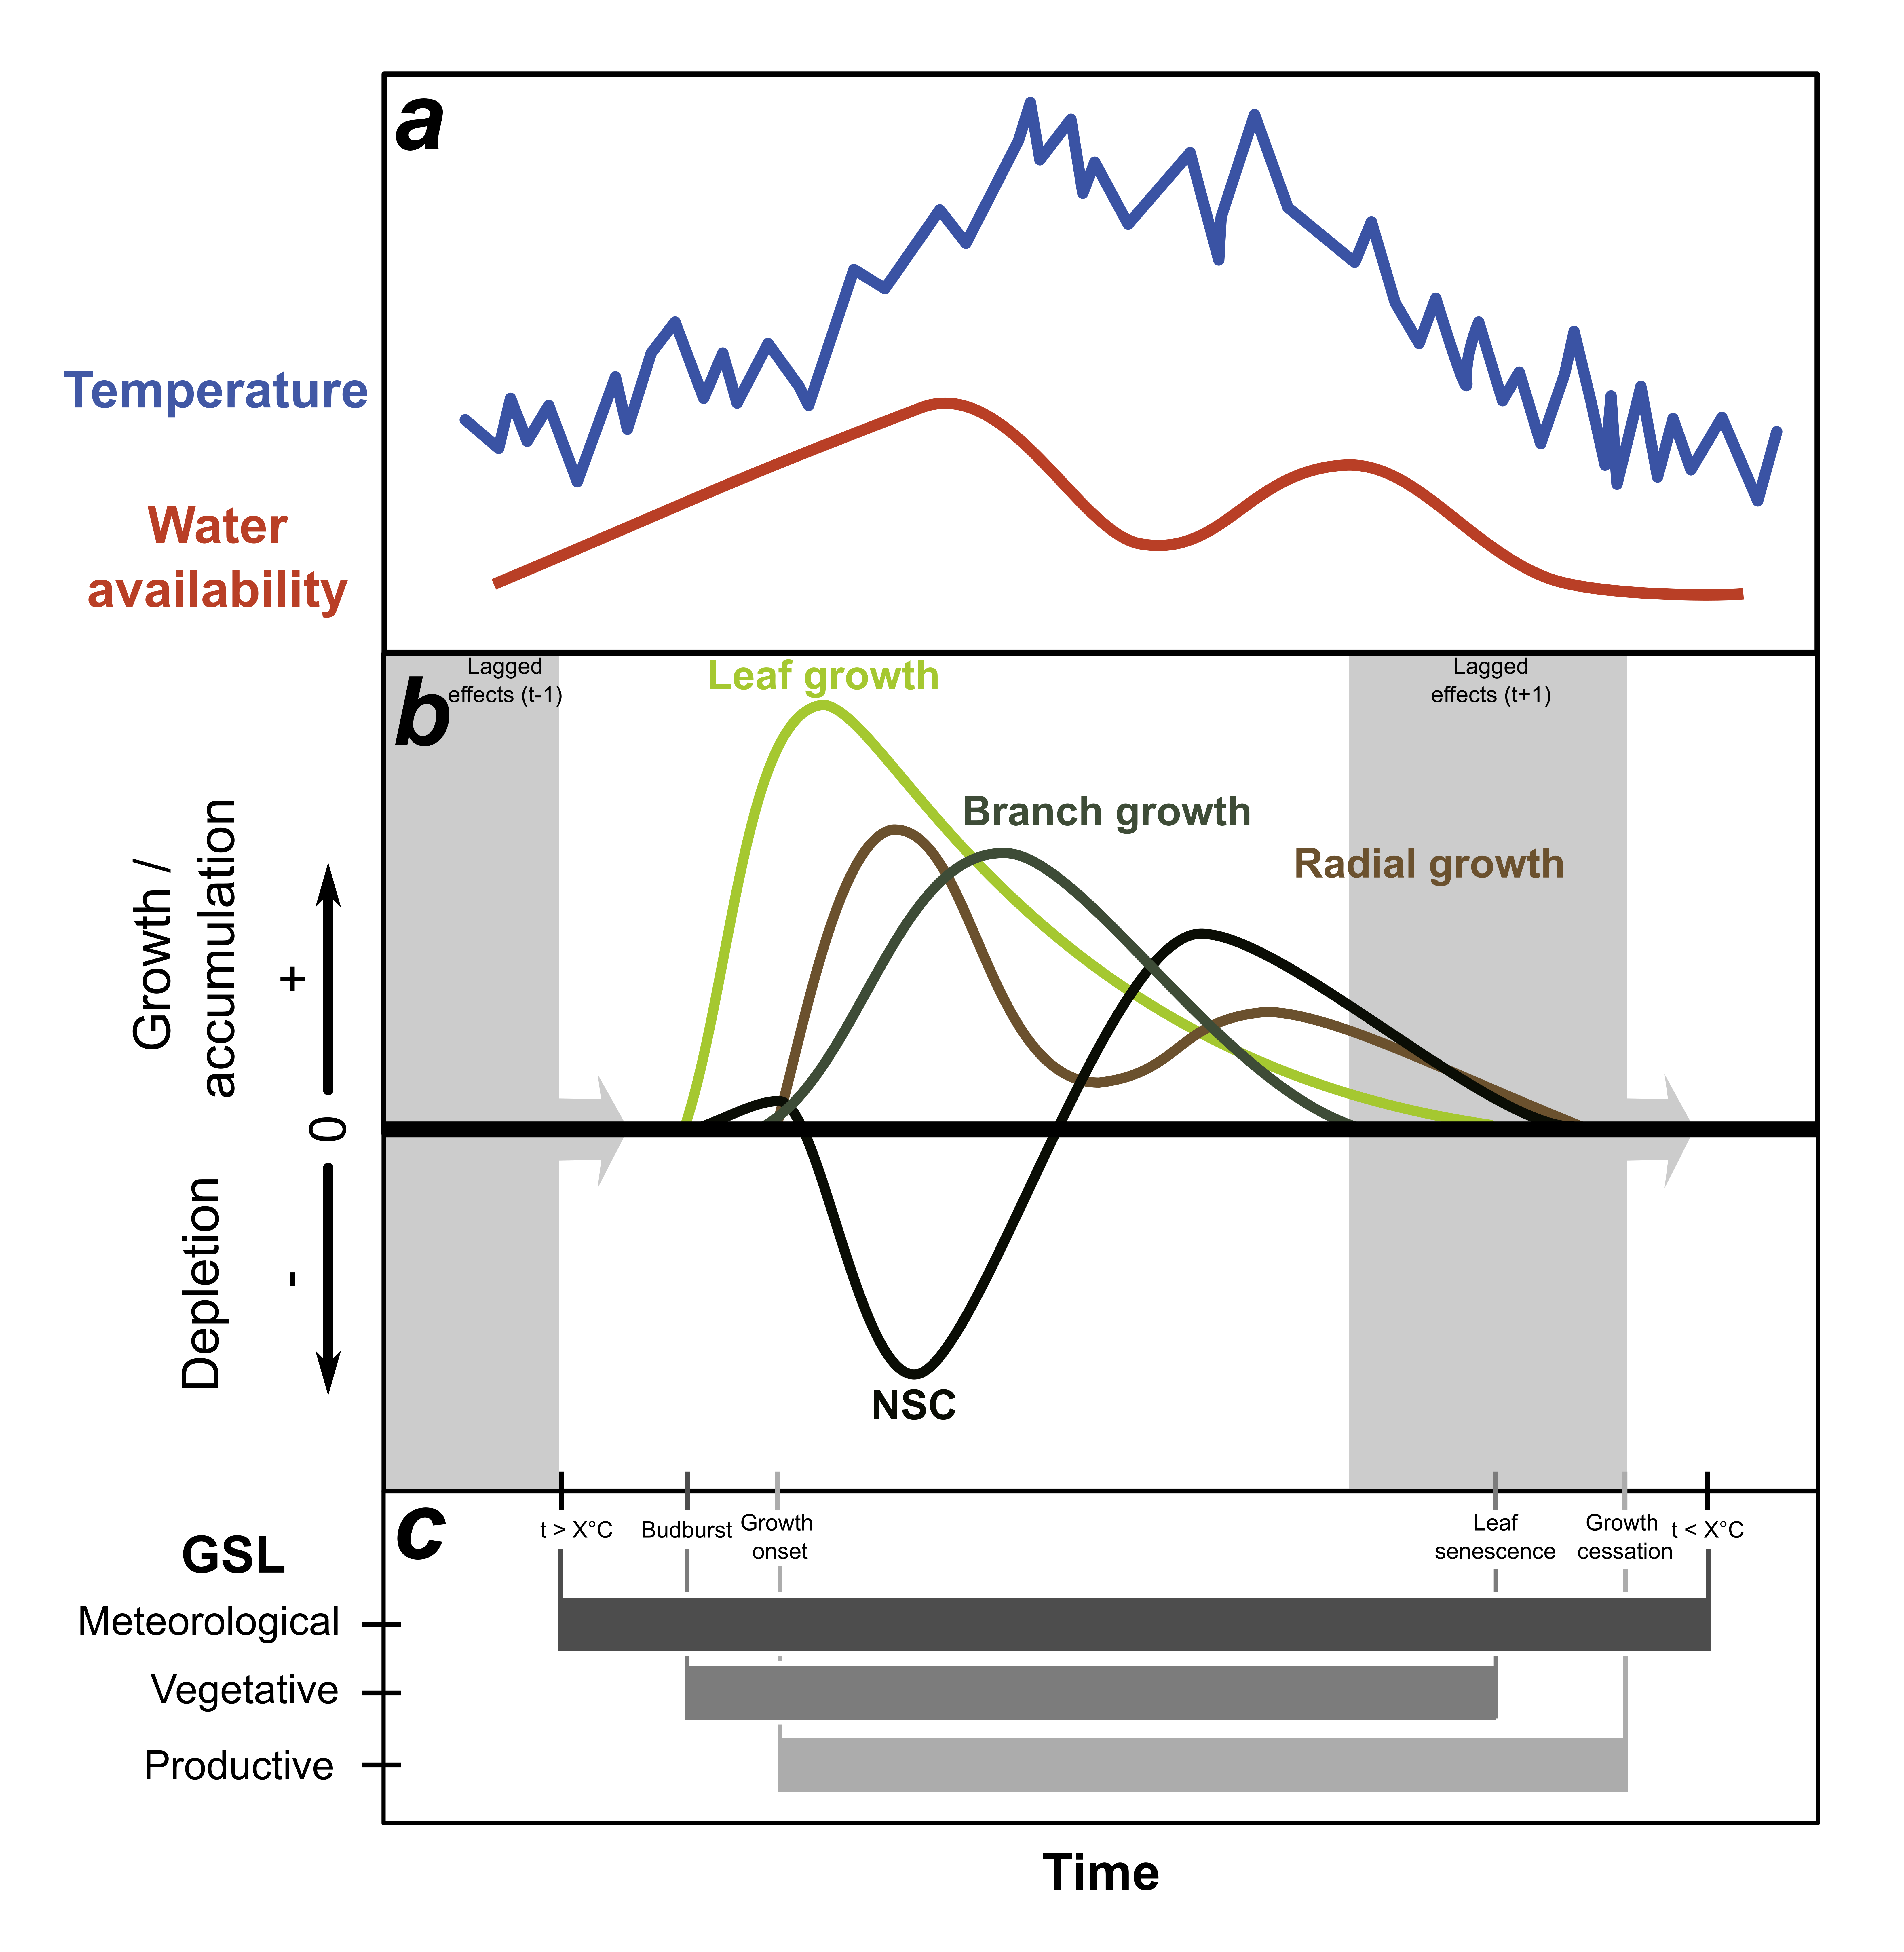
\includegraphics[width=0.5\textwidth]{..//figures/gslconcept/New_figure_growths.png}
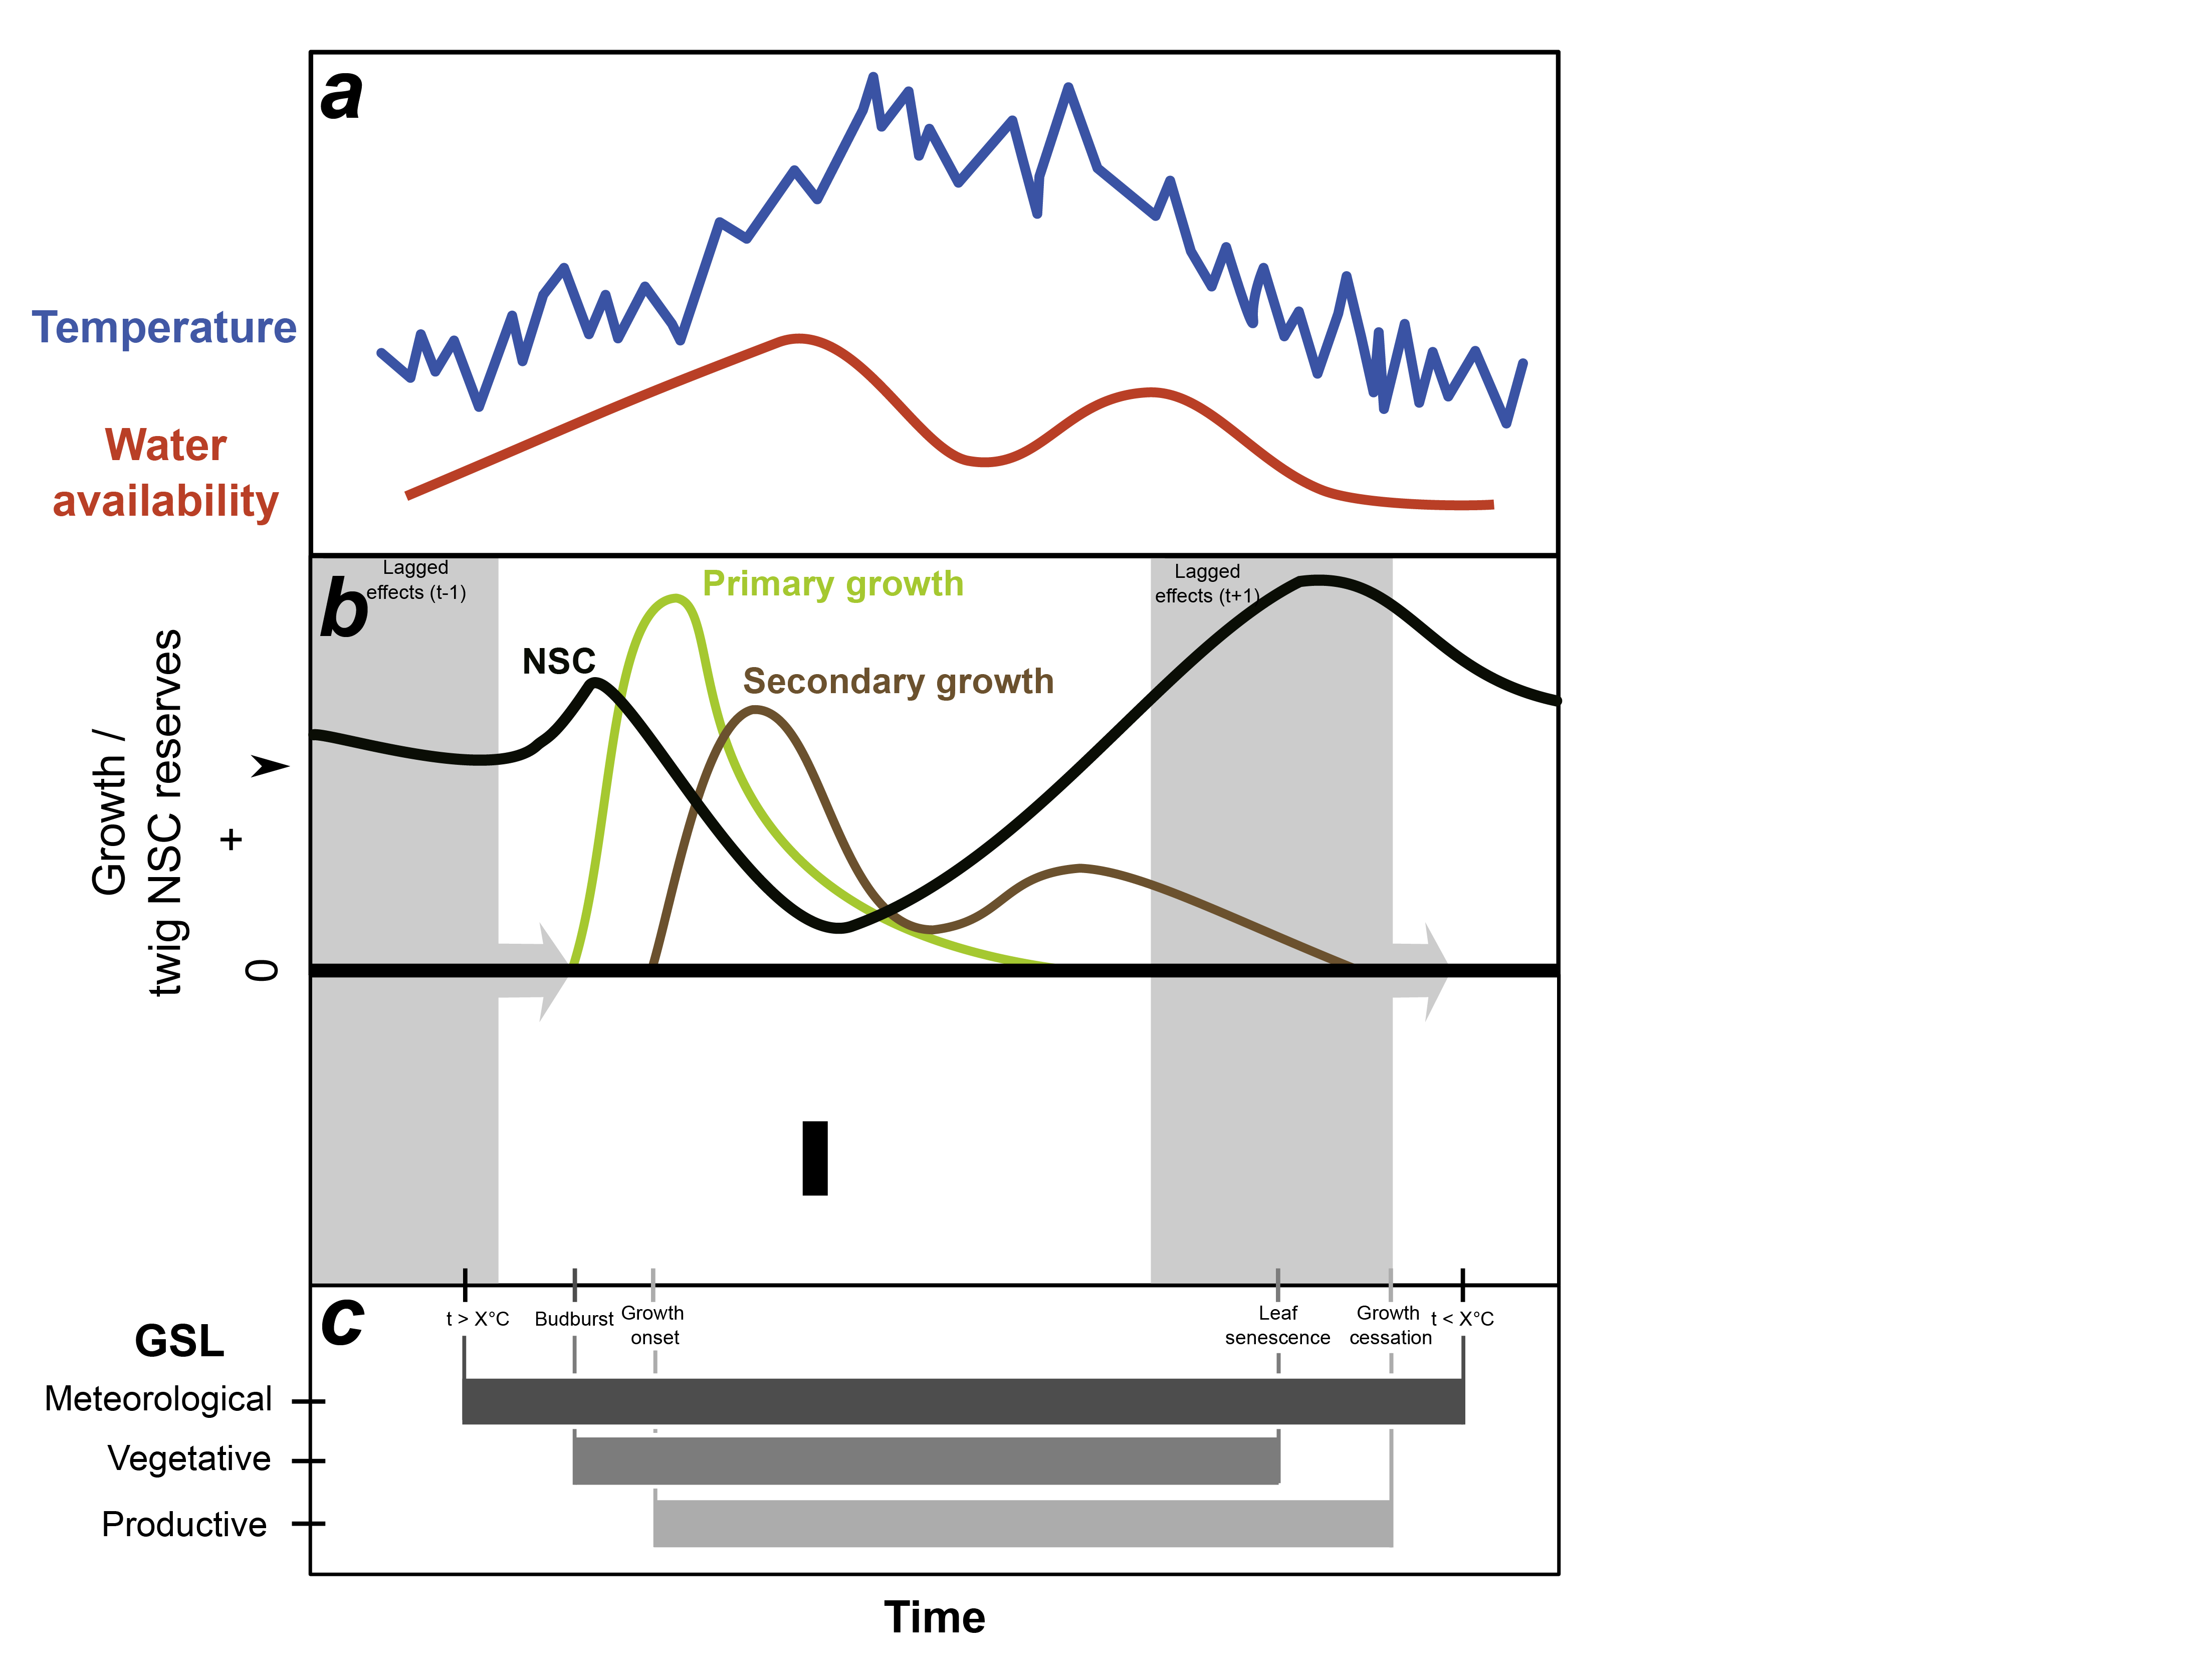
\includegraphics[width=0.7\textwidth]{..//figures/gslconcept/NEW_FI1_ac.png}
\caption{A major challenge in determining how growth responds to longer growing seasons is the complexity of each. Here we show the simplified climate of one year (a), which drives variation (b) in primary growth (root, shoot and leaf elongation) and secondary growth (radial wood growth), both of which often depend on growth from previous seasons. Each of these types of growth could define the growing season length (GSL, c) but similarly it can be defined meteorologically (e.g., days above 5\degree C with some level of soil moisture) or by large-scale measures of plant productivity \citep{korner2023four}. See also `The challenge of metrics: Measuring growth and growing season length' in the Supplement. [TWO versions of figure shown here currently---please comment if you have a strong preference.]]} 
\label{fig:defineGSLgrowth}
\end{figure}

\clearpage
\begin{figure}[h!]
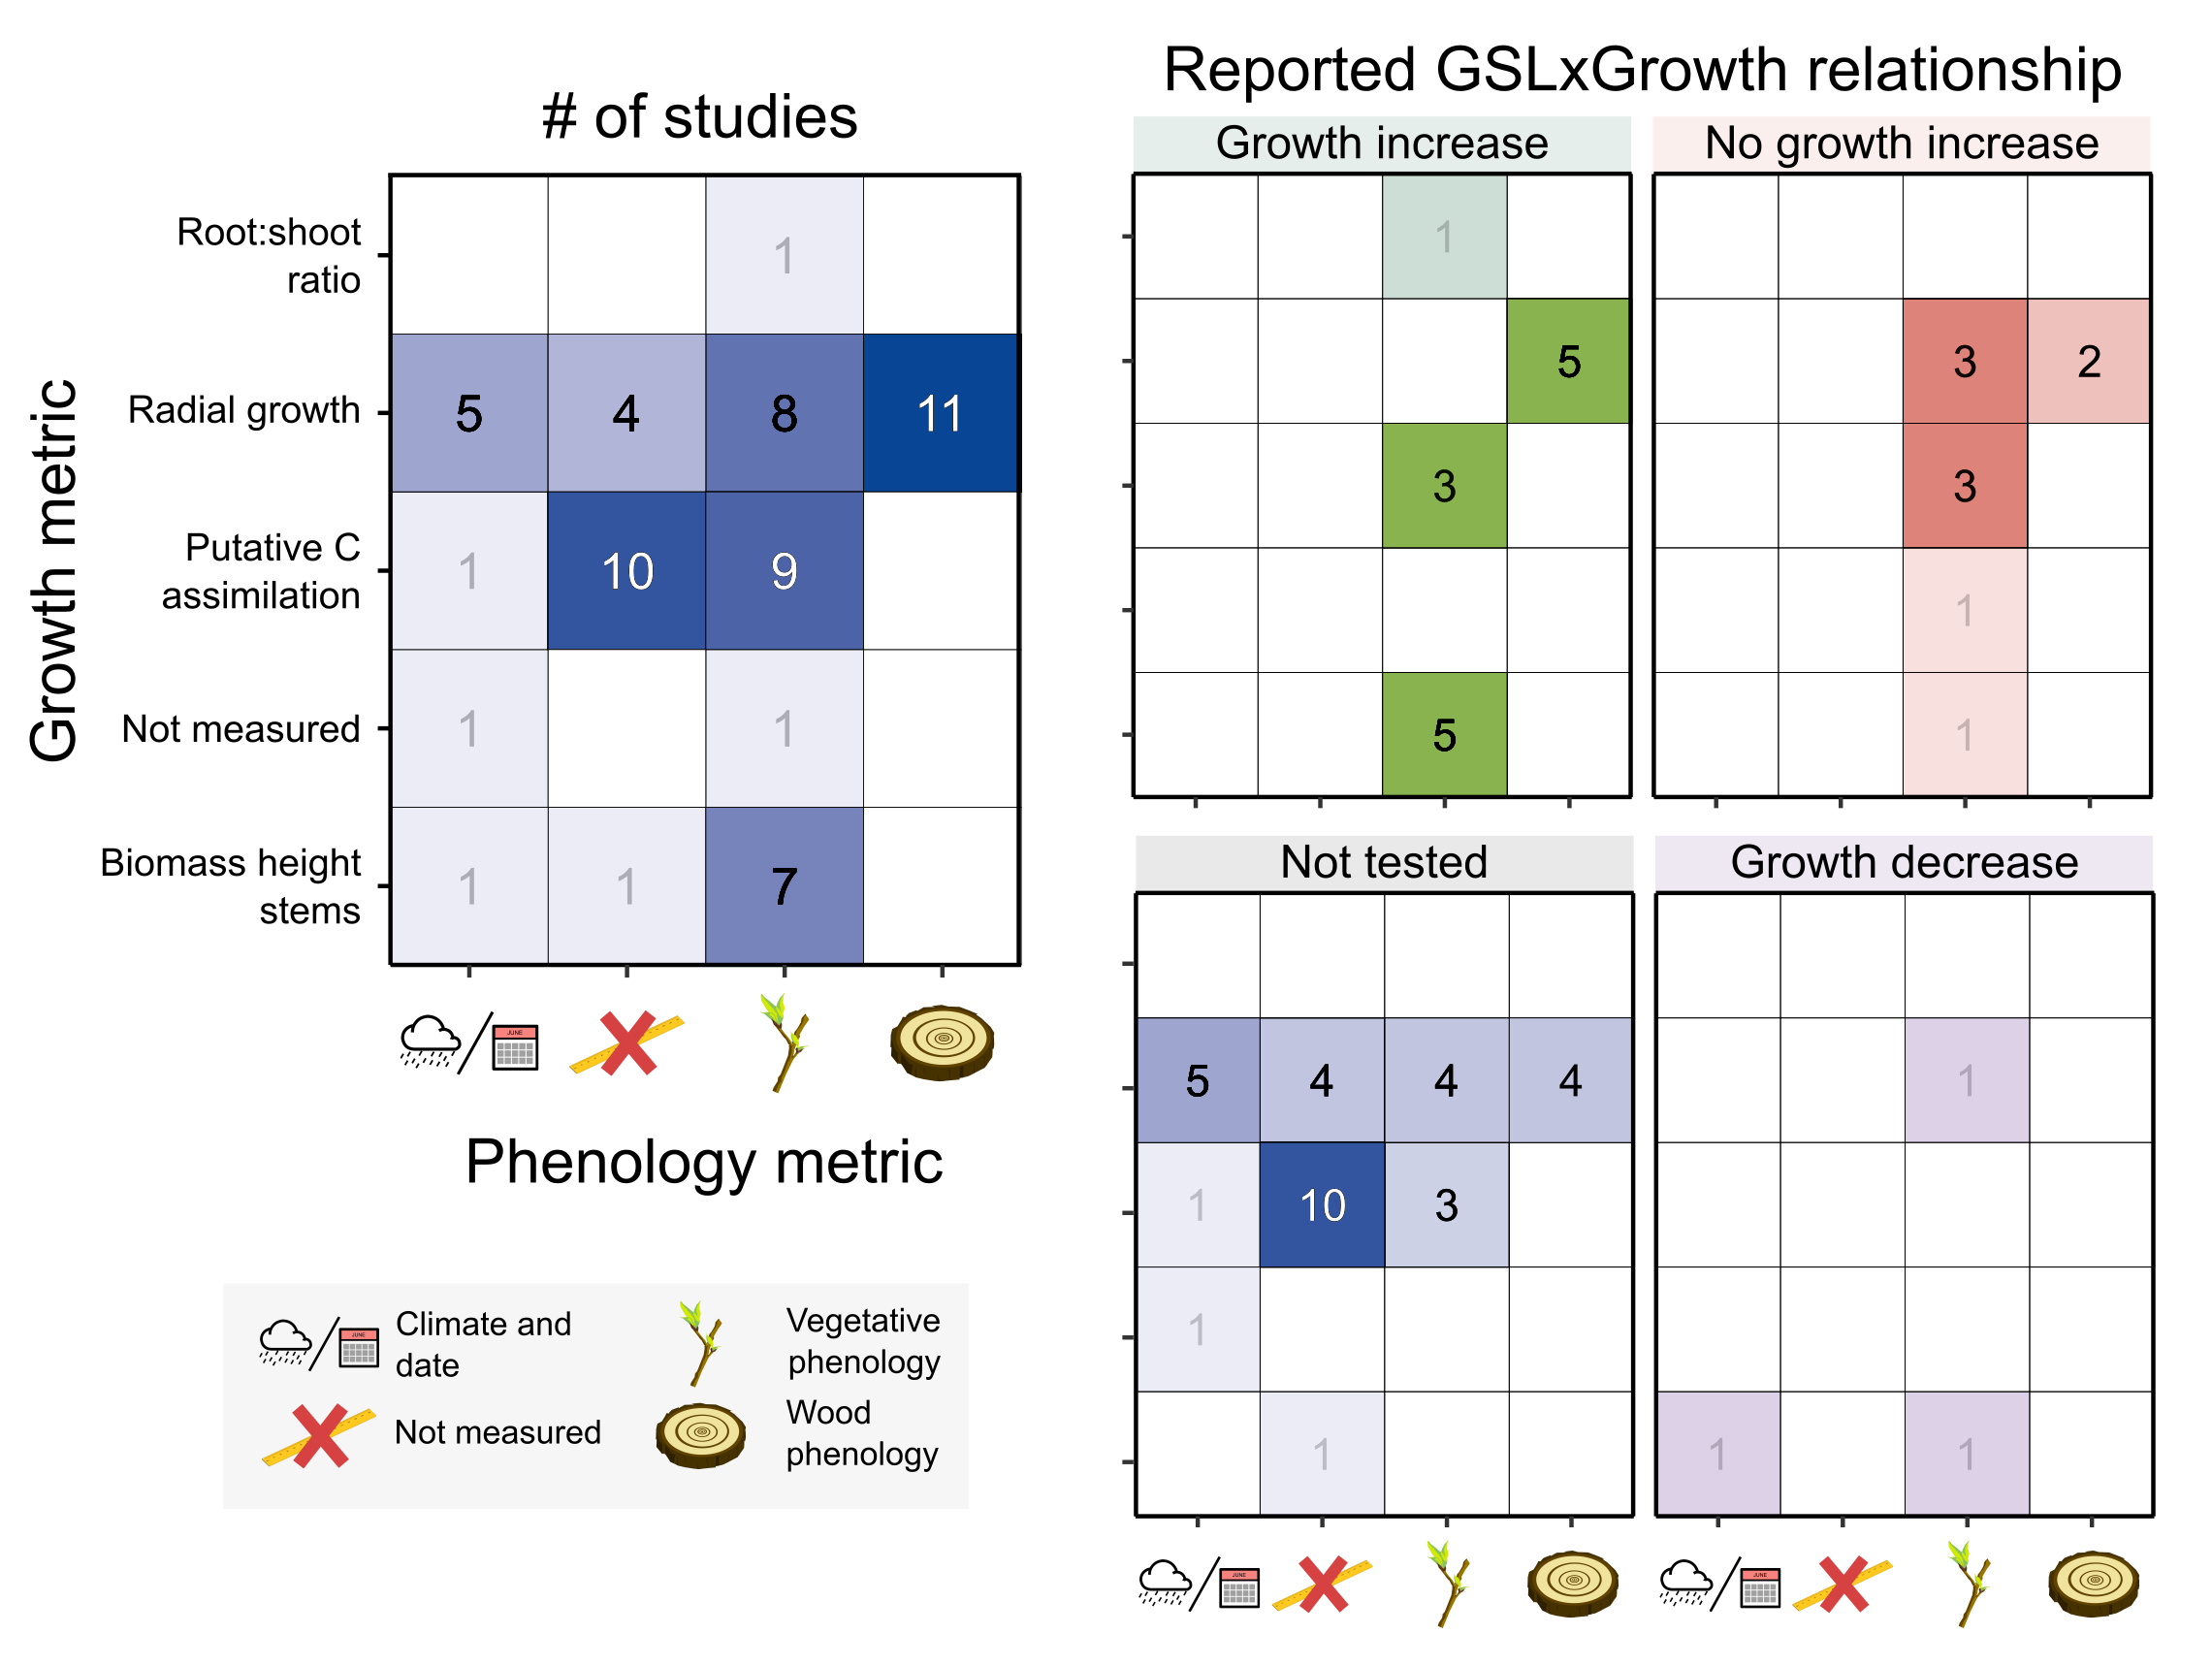
\includegraphics[width=1\textwidth]{..//figures/_figuresFromRuben/heatmap.png} % {..//figures/heatmaps/combinedheatmap_gslxgrowth_simple.pdf}
\caption{A review of growth $\times$ growing season length relationship studies spanned a diversity of methods, but there was no coherency in which methods did or did not find a positive relationship. A number of studies tested relationships possibly related to growth $\times$ growing season length (e.g., they tested how spring temperatures related to growth) but never directly growth $\times$ growing season length, thus `not tested' was surprisingly common across methods. See Supplement for review details.}
\label{fig:heatmaps}
\end{figure}


\begin{figure}[h!]
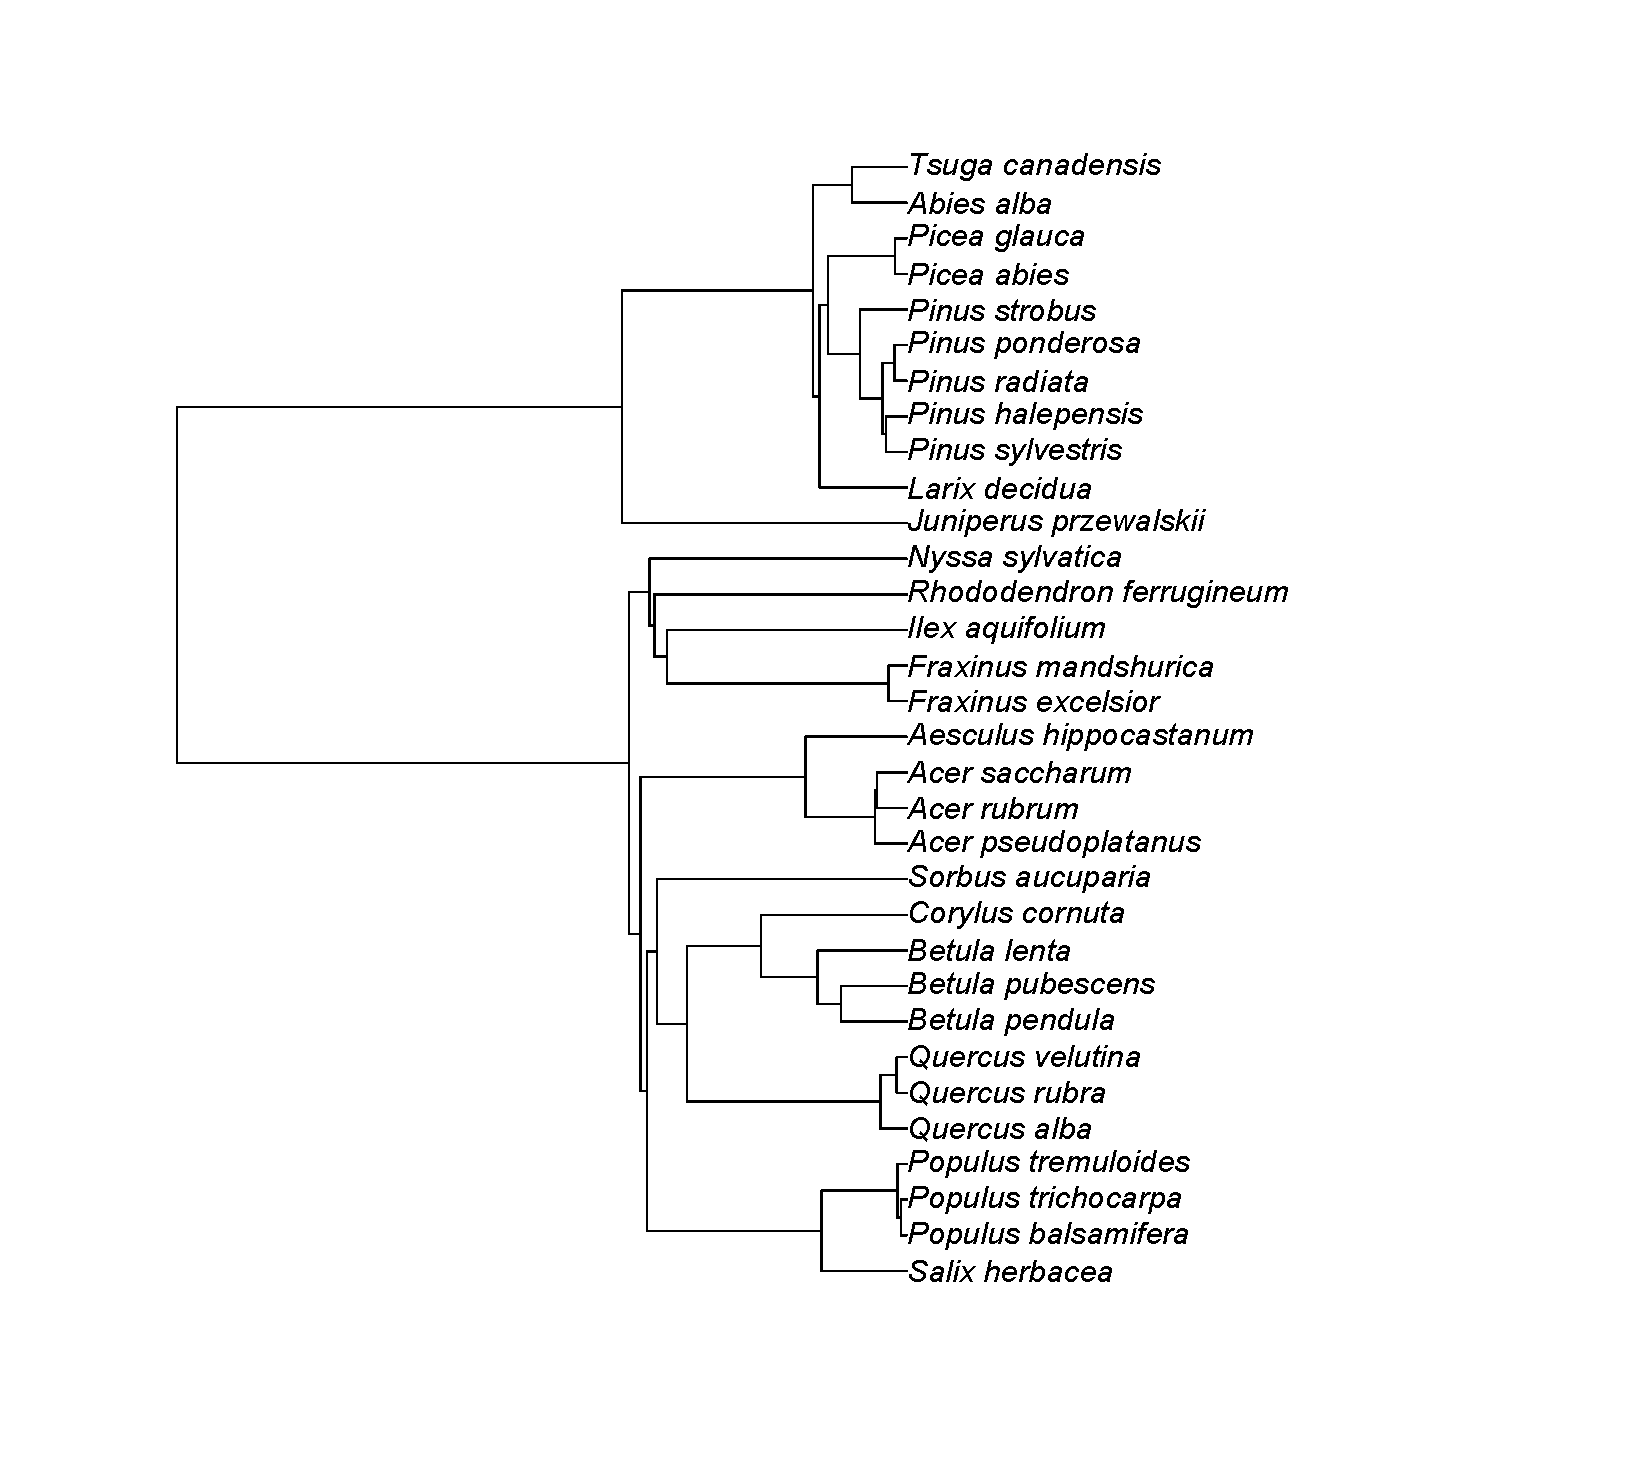
\includegraphics[width=1\textwidth]{..//figures/phylo.pdf}
\caption{We could switch Fig. \ref{fig:sppfinds} from Supp to main text and plot on phylogeny ... I just had time to plot the phylogeny quickly so did not layer on yes/no or find the missing species, like Fagus.}
\label{fig:sppphylo}
\end{figure}



\clearpage
\begin{figure}[h!]
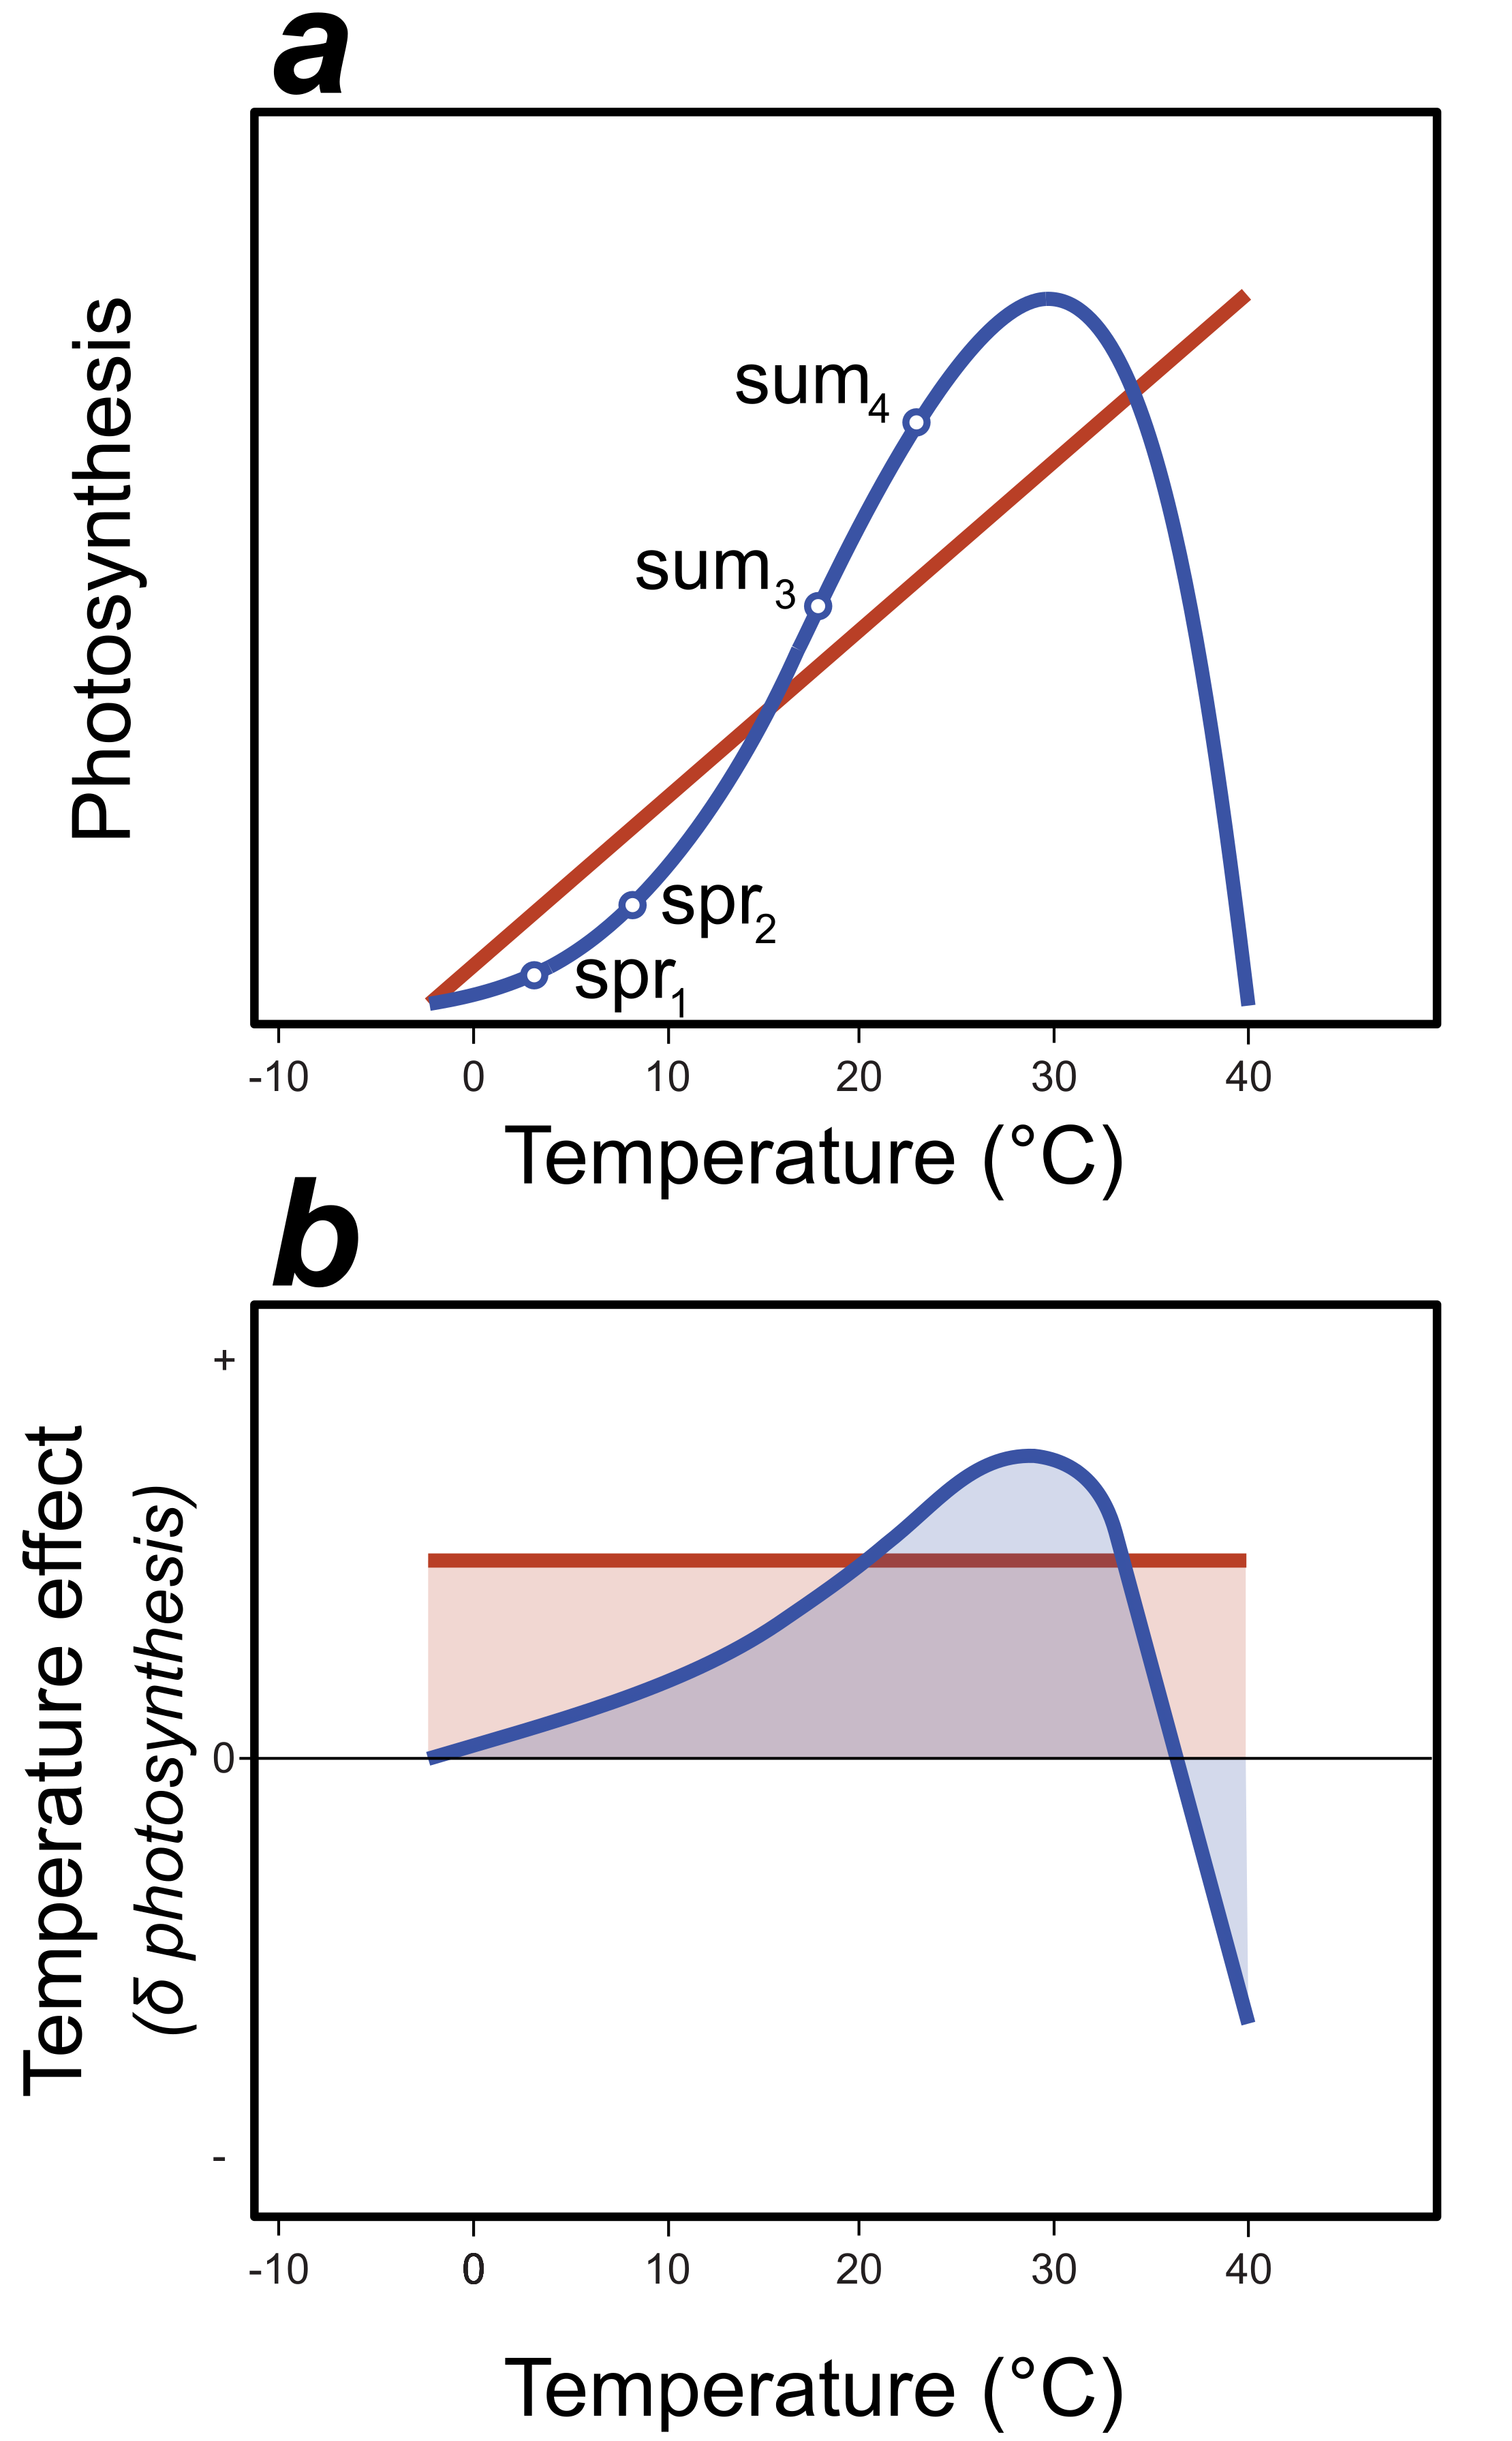
\includegraphics[width=0.5\textwidth]{..//figures/_figuresFromRuben/Tempresponses.png} %{..//figures/tempresponse/drafttempfig.png}
\caption{(a) Growth responses to temperature depends on a suite of complex factors and is often represented as net photosynthesis, which has a non-linear response to temperature  \citep[blue curve, adapted from meta-analysis of][]{rezende2019thermal}, though it is often modeled as linear (red). (b) This non-linearity means that increases in lower temperatures---such as those in the spring when much of growing season extensions may happen---have lower absolute increases in photosynthesis compared to increases in later-season (e.g., summer) warmer temperatures, while a linear response assumes a constant scale of effect across low to high temperatures.}
\label{fig:temperaturecomplex}
\end{figure}

\clearpage
\begin{figure}[h!]
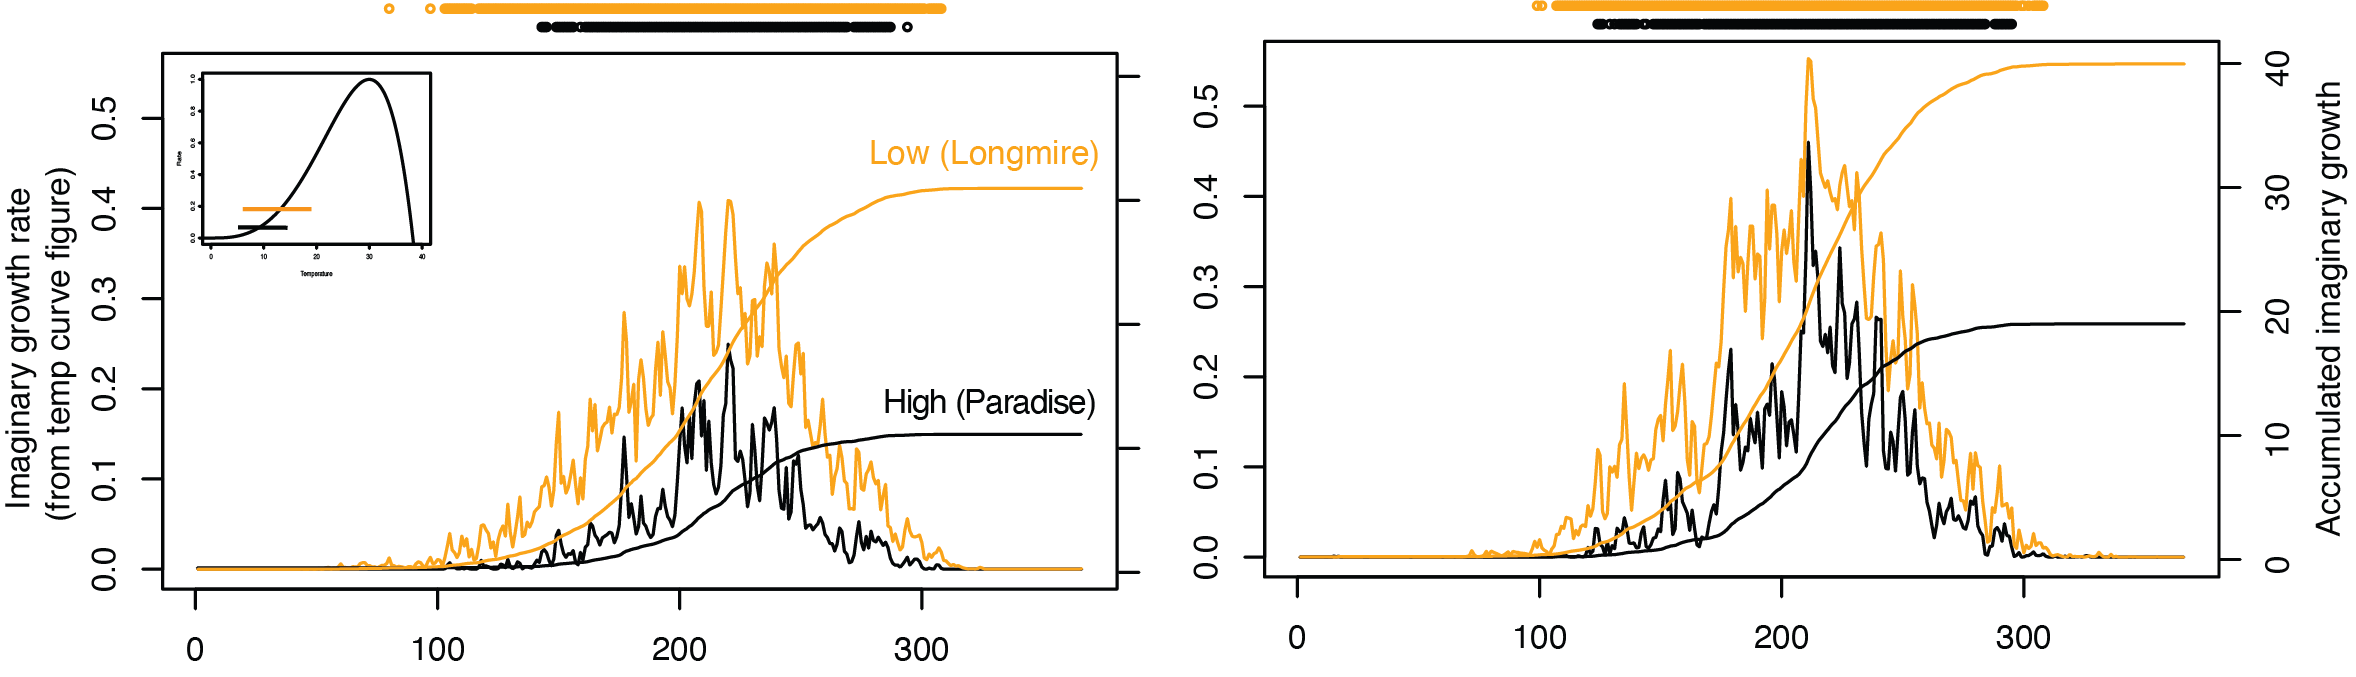
\includegraphics[width=1\textwidth]{..//figures/elevationconcept/elevationrates.png}
\caption{(DRAFT of potential new figure): Testing how growth varies across larger spatial gradients of growing season length could help establish a baseline expectation of the scale of temporal---especially inter-annual variation---and force a greater reckoning with drivers that shift alongside growing season length. This conceptual figure uses data from a cool-weather, temperate site at two elevations (Mount Rainier/Tahoma in USA) with show potential differences in growing season length (dots on top) and biological rates. Other gradients in warmer locations would show much higher rates, but also likely more days where rates are zero due to too high temperatures. Here we estimated growing season length as days above 5\degree C and used an idealized curve (inset) to calculate daily rates. Left shows based on climatic data from the 1980s, while the right is based on 2014-2023. [I could edit this to show TWO species that respond slightly differently to temperature, but then we need to drop one elevation or one time period. THOUGHTS?] }
\label{fig:moraconcept}
\end{figure}

\clearpage
\begin{figure}[h!]
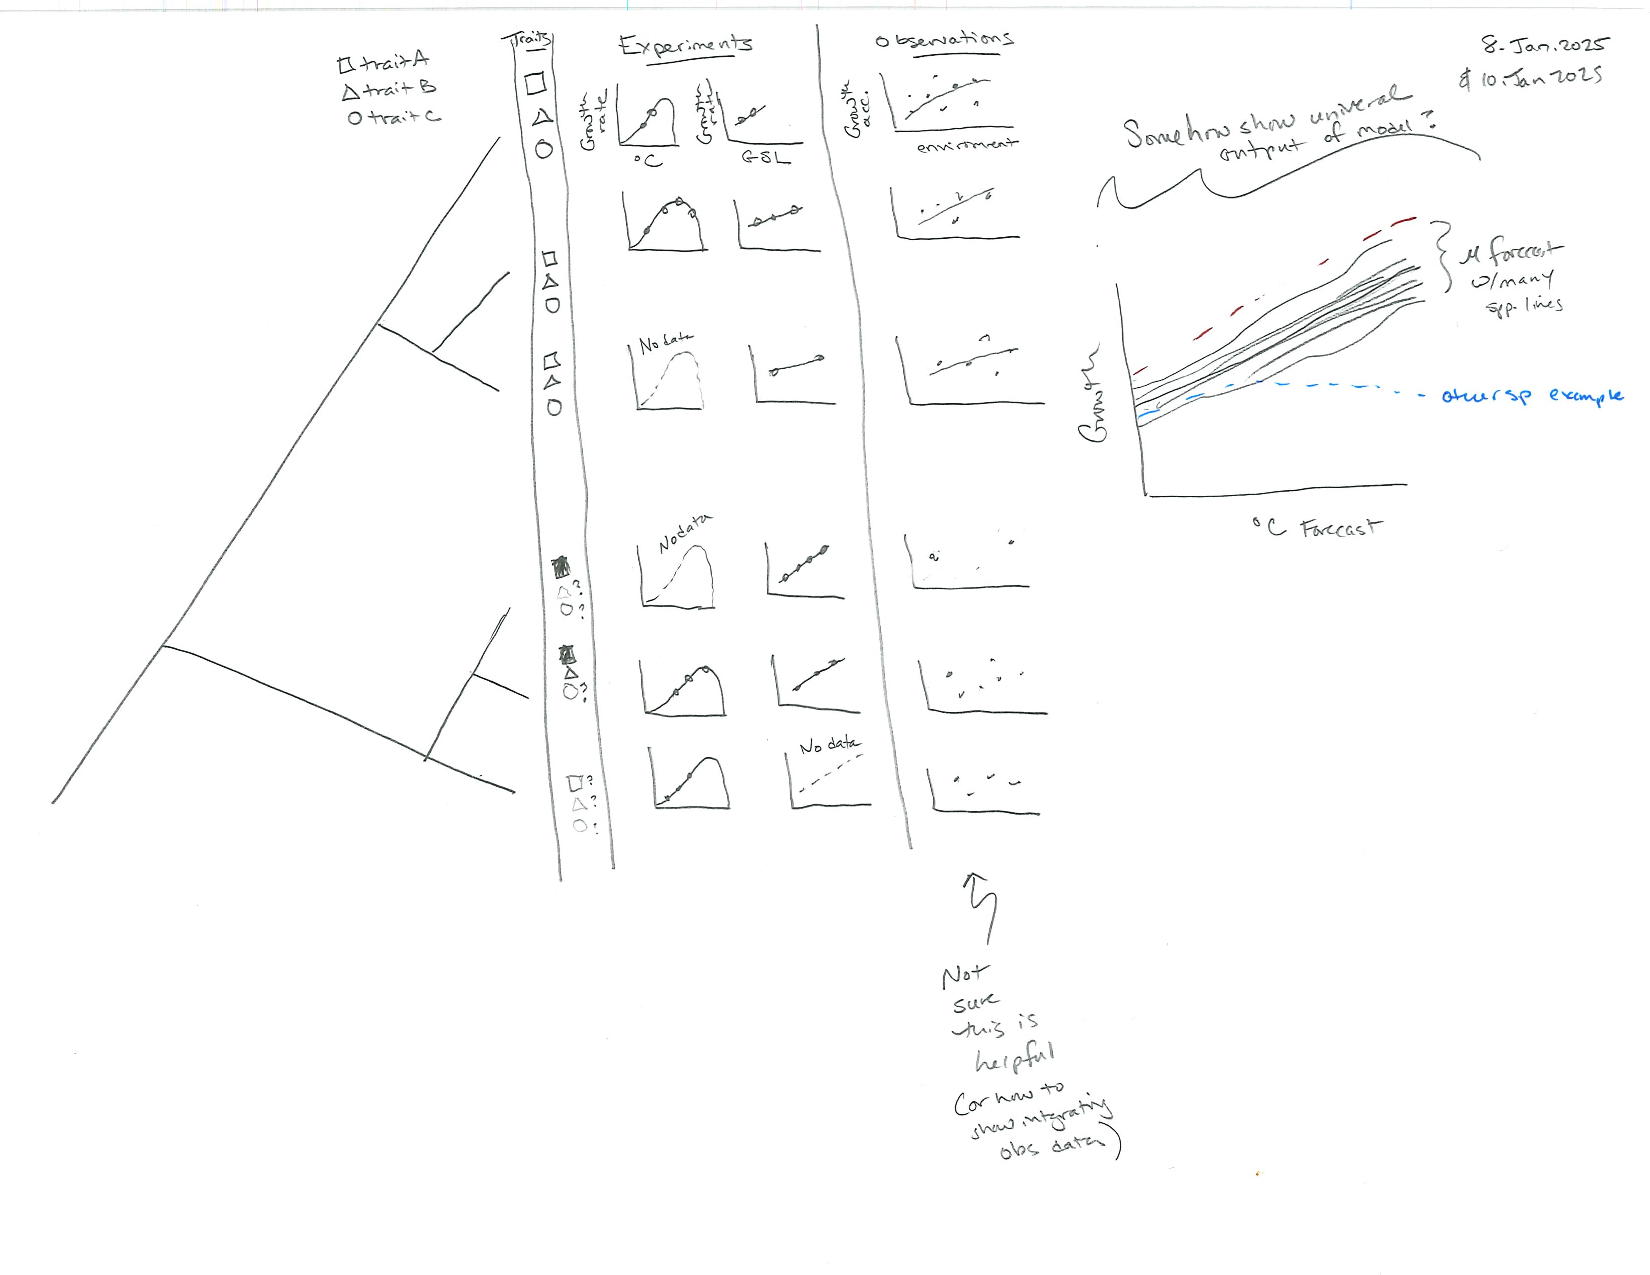
\includegraphics[width=1\textwidth]{..//figures/phylomodel/2025Jan8_conceptphylomodel.pdf}
% JHRL: When you say universal output of a model - what do you mean? A forecast of how an entire forest responds?
% Maybe there you can add to this right panel two more boxes / graphs - one showing a hypothetical forest including these species, subjected to a CC forecast and the output of this model?
\caption{(DRAFT of potential new figure): A trait-based phylogenetic model provides a way to naturally organize species (and, not shown, population) responses to predict how they will respond to longer seasons. This approach leverages species shared evolutionary history (shown at left via a phylogenetic tree) to produce a universal model across species while also predicting how each species should uniquely respond while handling unevenness in sampling and missing data (the `no data' curves represent that the model will predict a curve for each species, informed to various degrees---with the degree determined by the model---by the traits and phylogeny). In this example, we show how this approach can identify one clade (top) with a common response to longer seasons that also shares a suite of similar traits, and can identify a unique response in by one species in a clade where that species also has a unique trait compared to other species with the same common ancestor (lower clade -- ACTUALLY, I do not sow this, but could).}  % Similarly traits that co-vary with different responses can be more quickly identified by identifying the common ancestor to species with similar responses!
\label{fig:phylomodel}
\end{figure}

\clearpage
\begin{figure}[h!]
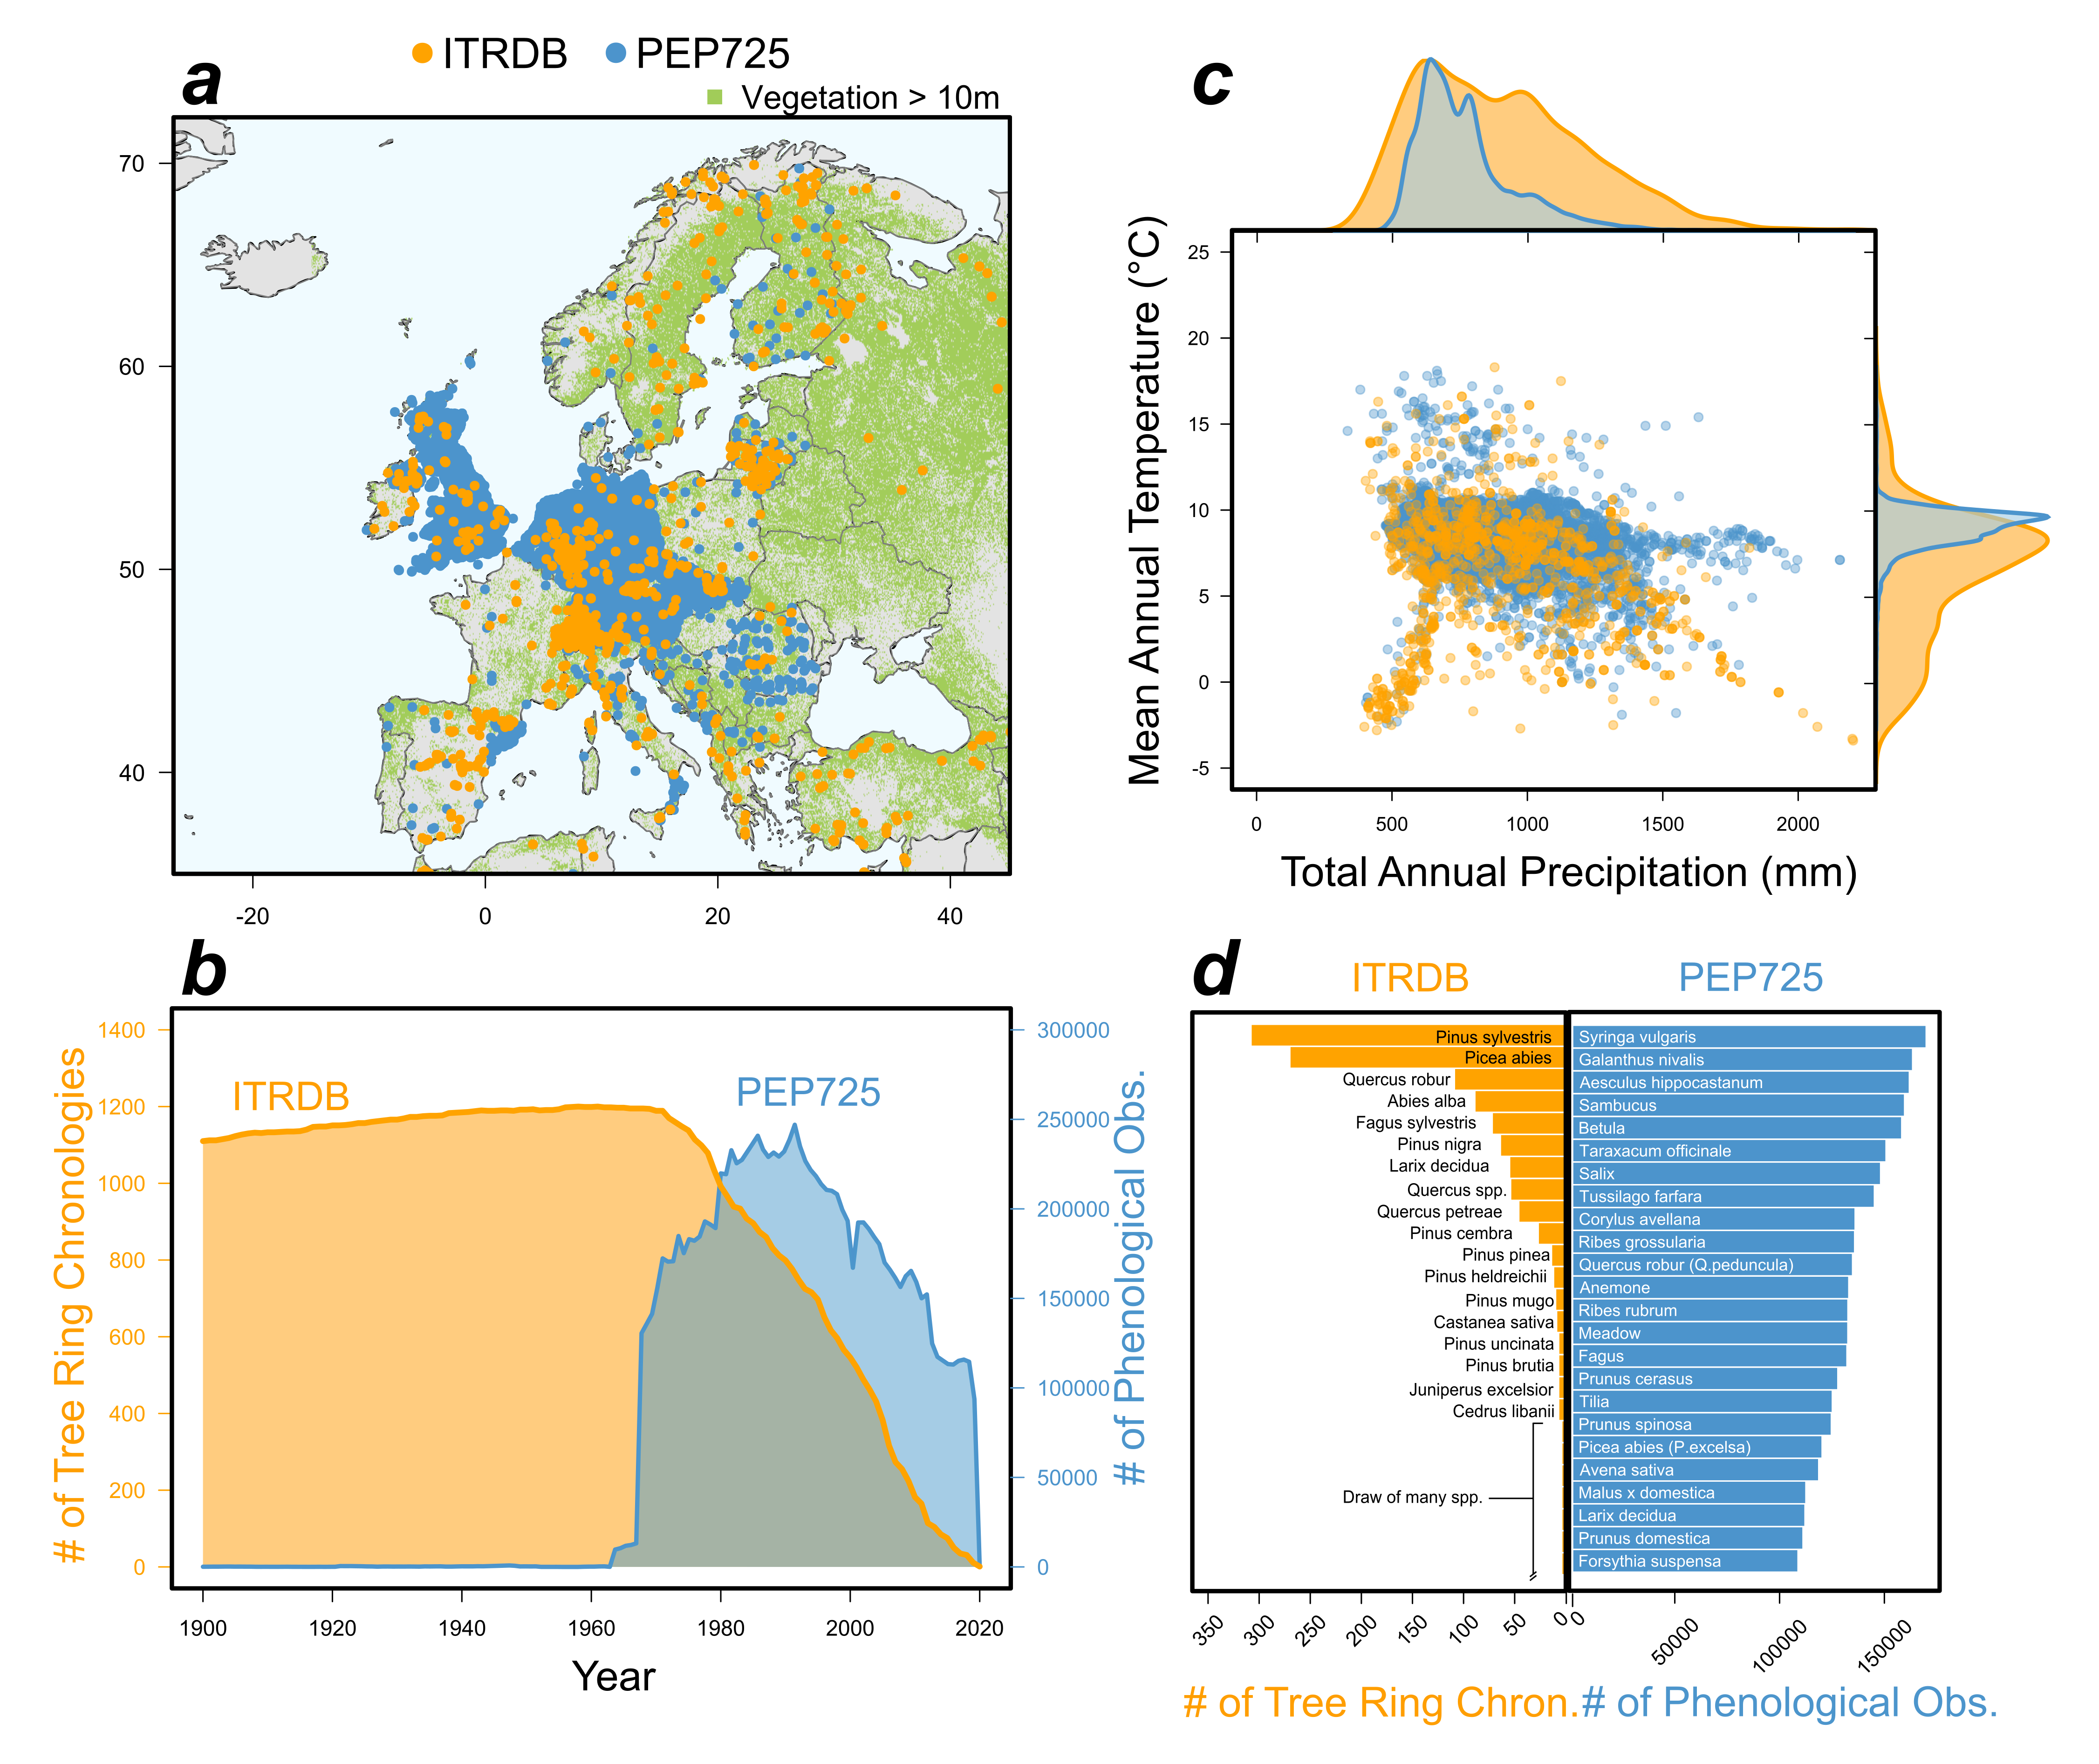
\includegraphics[width=1\textwidth]{..//figures/_figuresFromRuben/itrdb_vs_pep.png} %{..//figures/itrdbpep.png}
\caption{Data overlap between the two major databases of growth (International Tree Ring Data Bank, ITRDB, orange) and plant phenology (Pan European Phenology Project, PEP725, blue). Both databases are compared in terms of their spatial distributions (a), temporal overlaps (b), coverage of environmental conditions in climate space (c) and taxonomical representation (d). Note that the number of tree ring chronologies in (b) are composed by multiple trees per site, typically 10-20. Climatic data from Worldclim database ver. 2.1 at 2.5\degree grid resolution. PEP725 records in d) show the largest records for any given phenophase per species.}
\label{fig:itrbdpep}
\end{figure}


\end{document}
